ABAI can be broken down into two smaller programs. You will be able to use the \textbf{local application} if you want to customize the data, the models and their feature extraction processes. The \textbf{web based application} is a simplified tool that uses pre-trained models to perform the authorship attribution task based on the model you select. 

\subsection{Local application}
The GUI for the local application consists of a main application window and is then divided into multiple sub-windows for each menu option. If you close the main window or any sub-window, their child windows will also be closed. 
\begin{center}
    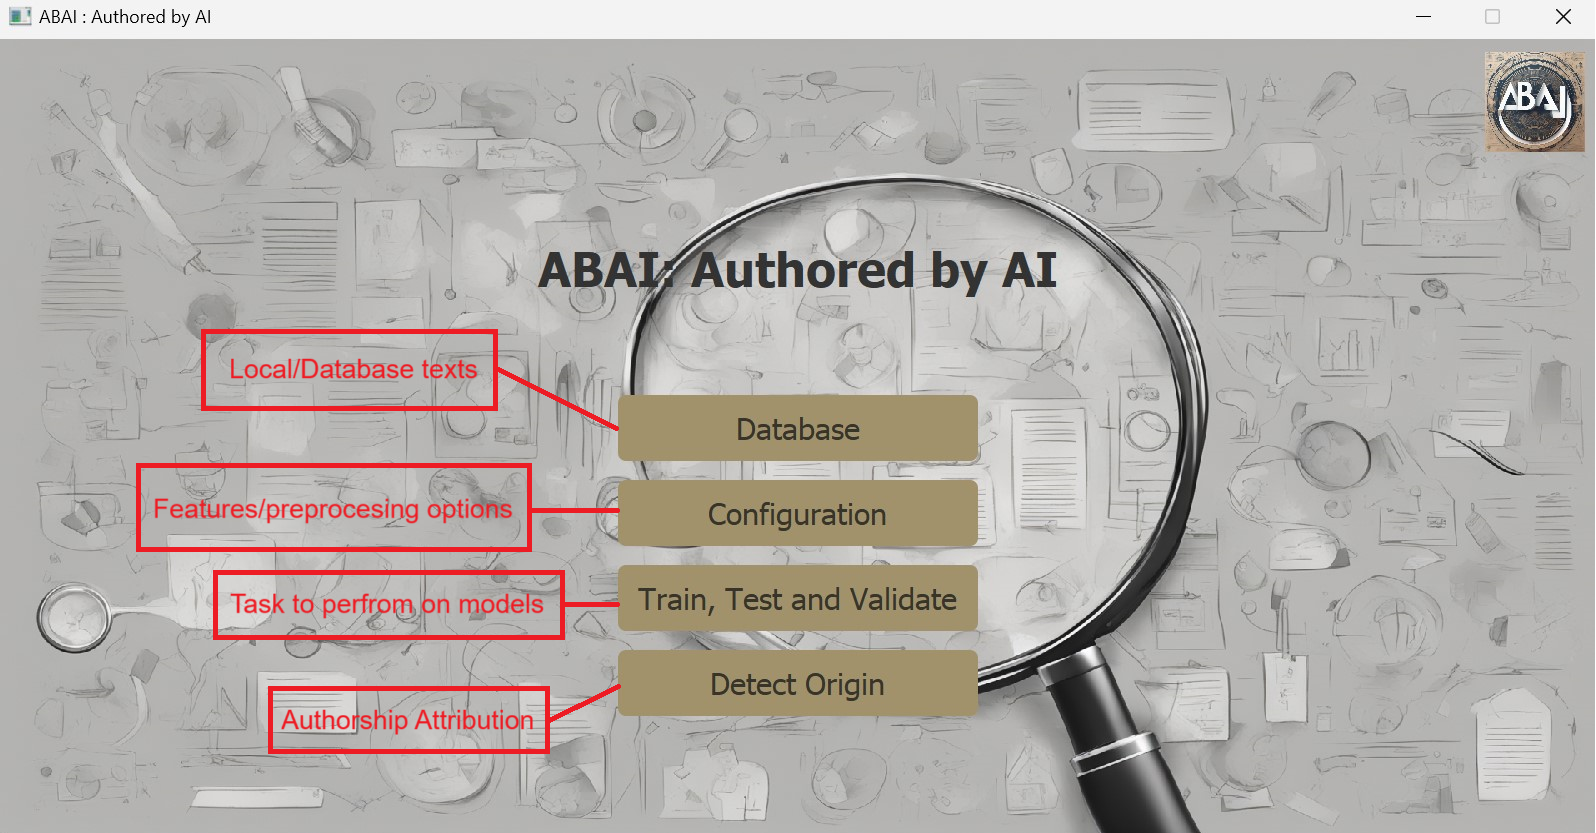
\includegraphics[width=17cm]{Images/Usage/Local/MainWindow.png}
\end{center}
Now, let's break down the menu and it's options into smaller parts further explained in the following sections.
\clearpage
\subsubsection{Database}
\label{subsubsec:database}
In the database sub-window, you will be able to modify everything related to the databases and local files ABAI will draw from during the training of it's models. It's possible to add/remove directly to/from the \texttt{SQLite} database as well as storing local \texttt{.TXT} files. 
\begin{center}
    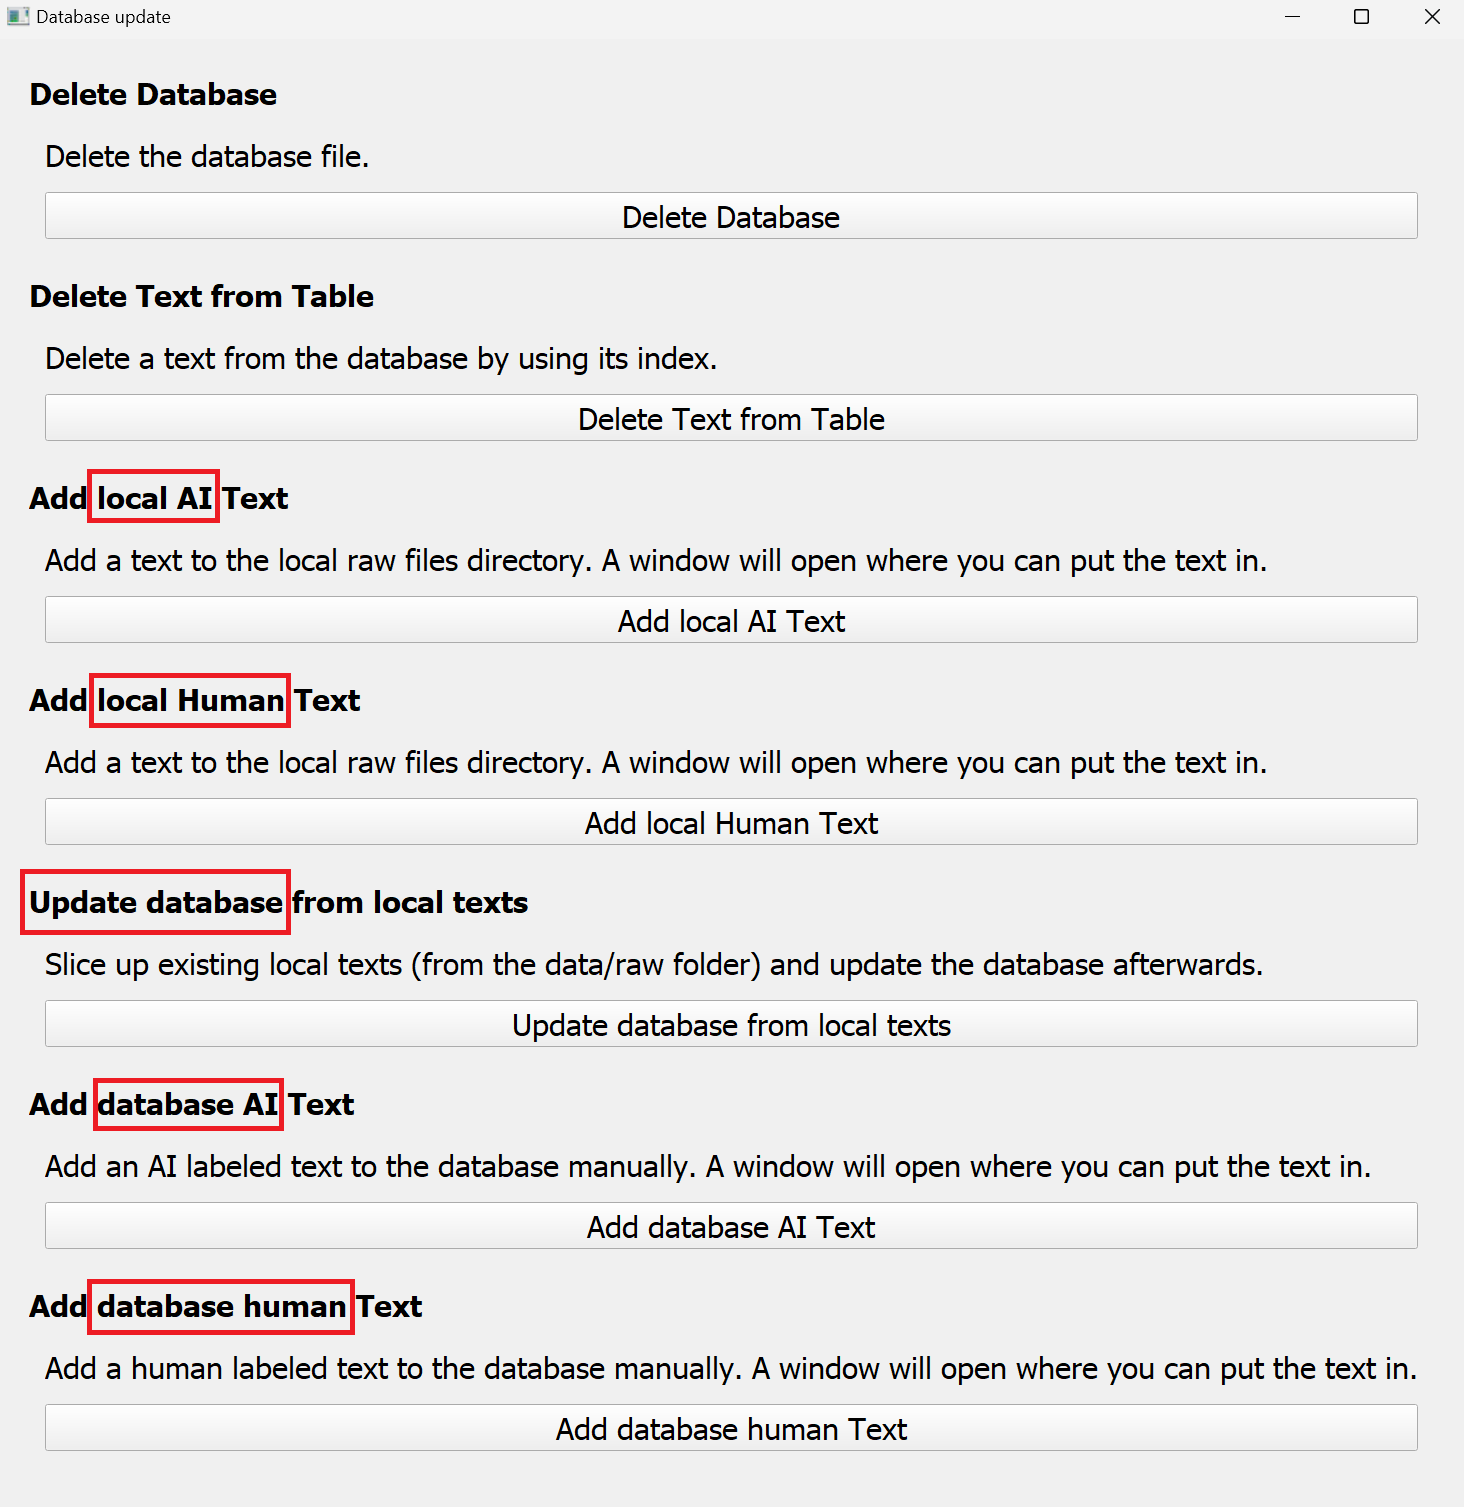
\includegraphics[width=17cm]{Images/Usage/Local/DatabaseWindow.png}
\end{center}
\clearpage
\subsubsection{Configuration}
In the configuration sub-window, you will be able to set options for different methods of feature extraction, cross-validation and random state used during processing tasks. 
\begin{center}
    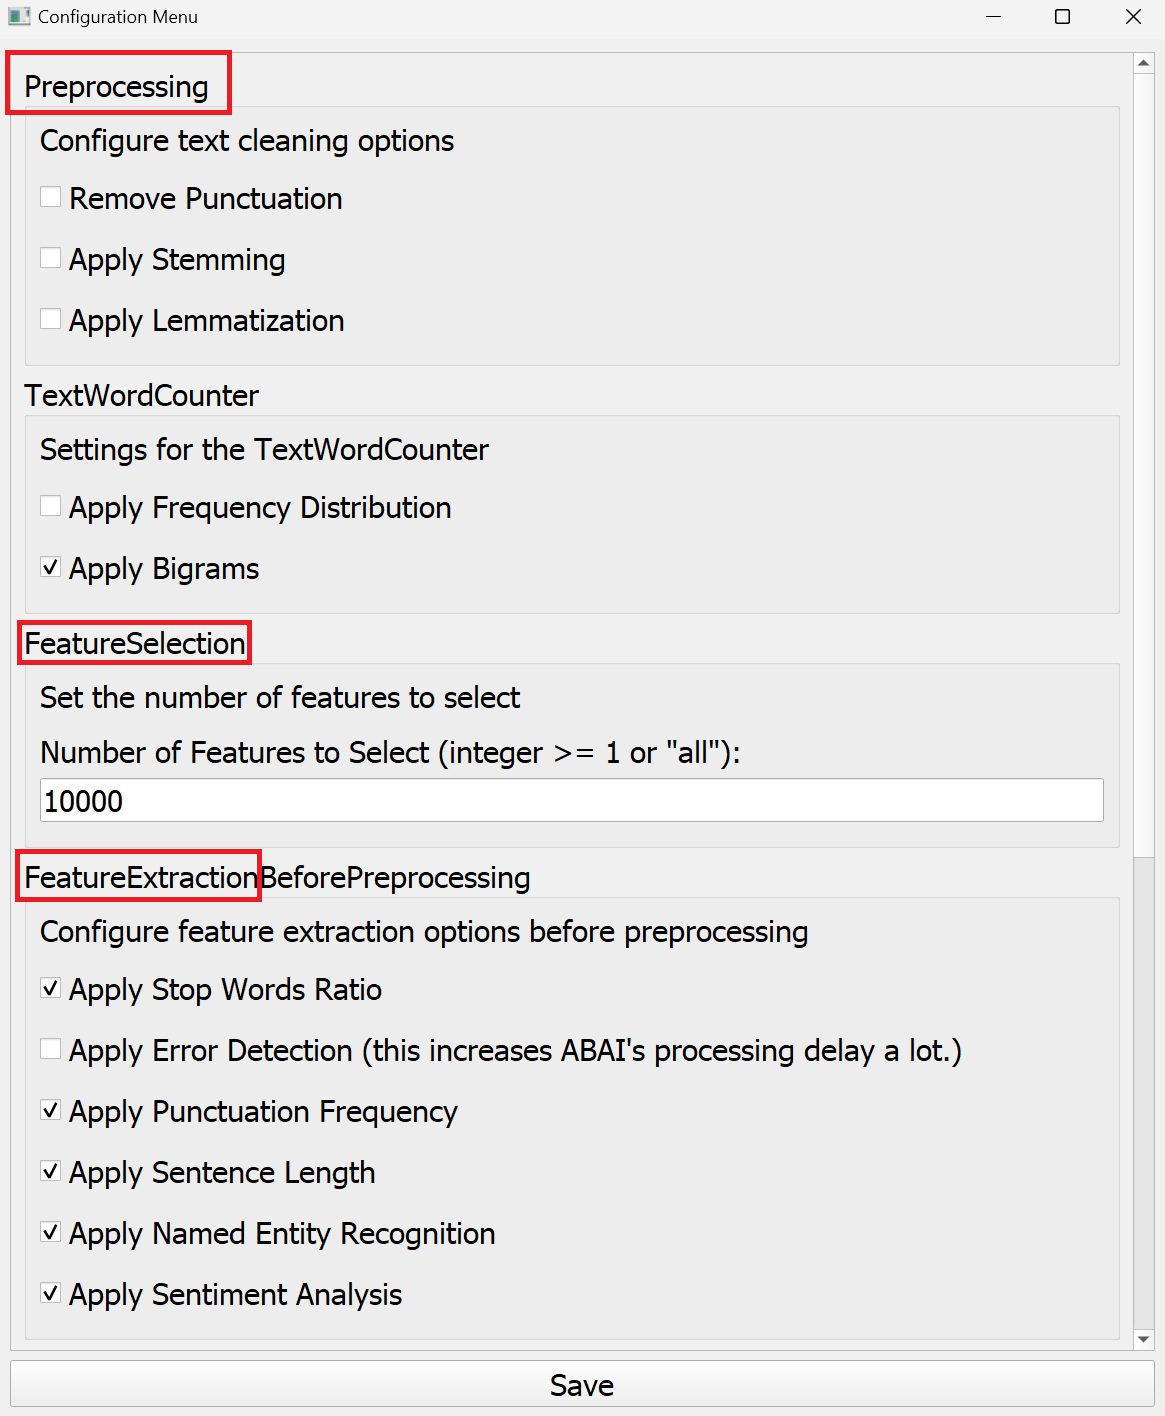
\includegraphics[width=17cm]{Images/Usage/Local/ConfigurationWindow.png}
\end{center}
\clearpage
\paragraph{\fontsize{14}{17}\selectfont A brief explanation}
\label{subsubsec:config-brief-explain}
\begin{itemize}
    \item \textbf{Preprocessing}\\\\
    Configure the text cleaning options. These options include removing punctuation, applying stemming, and lemmatization.\\
    
    \item \textbf{TextWordCounter}\\\\
    Choose between frequency distribution or tf-idf calculation, as well as whether to include bigrams in addition to unigrams.\\
    
    \item \textbf{FeatureSelection}\\\\
    Specify the number of features to select for Kbest feature selection using the chi2 function. This setting allows you to control the dimensionality of your features.\\
    
    \item \textbf{FeatureExtractionBeforePreprocessing}\\\\
    This segment includes several feature extraction options that will be performed before preprocessing. These include applying stop words ratio, error detection for grammar and misspells (which may prolong the processing time because of API calls), punctuation frequency, average sentence length, named entity recognition, and sentiment analysis.\\
    
    \item \textbf{FeatureExtractionAfterPreprocessing}\\\\
    Apply additional feature extraction methods that will be performed after preprocessing. These include text word counting, average word length, and vocabulary size.\\
    
    \item \textbf{CrossValidation}\\\\
    Set the number of folds for cross-validation.\\
\end{itemize}

\subsubsection{Train, Test, and Validate}
\label{subsubsec:train-test-validate}
In the train, test and validate sub-window you will be able to select the models you want to use (multiple simultaneous selections are allowed) and which task you want to perform for them. After the task has finished, a new window will open with the result.
\begin{center}
    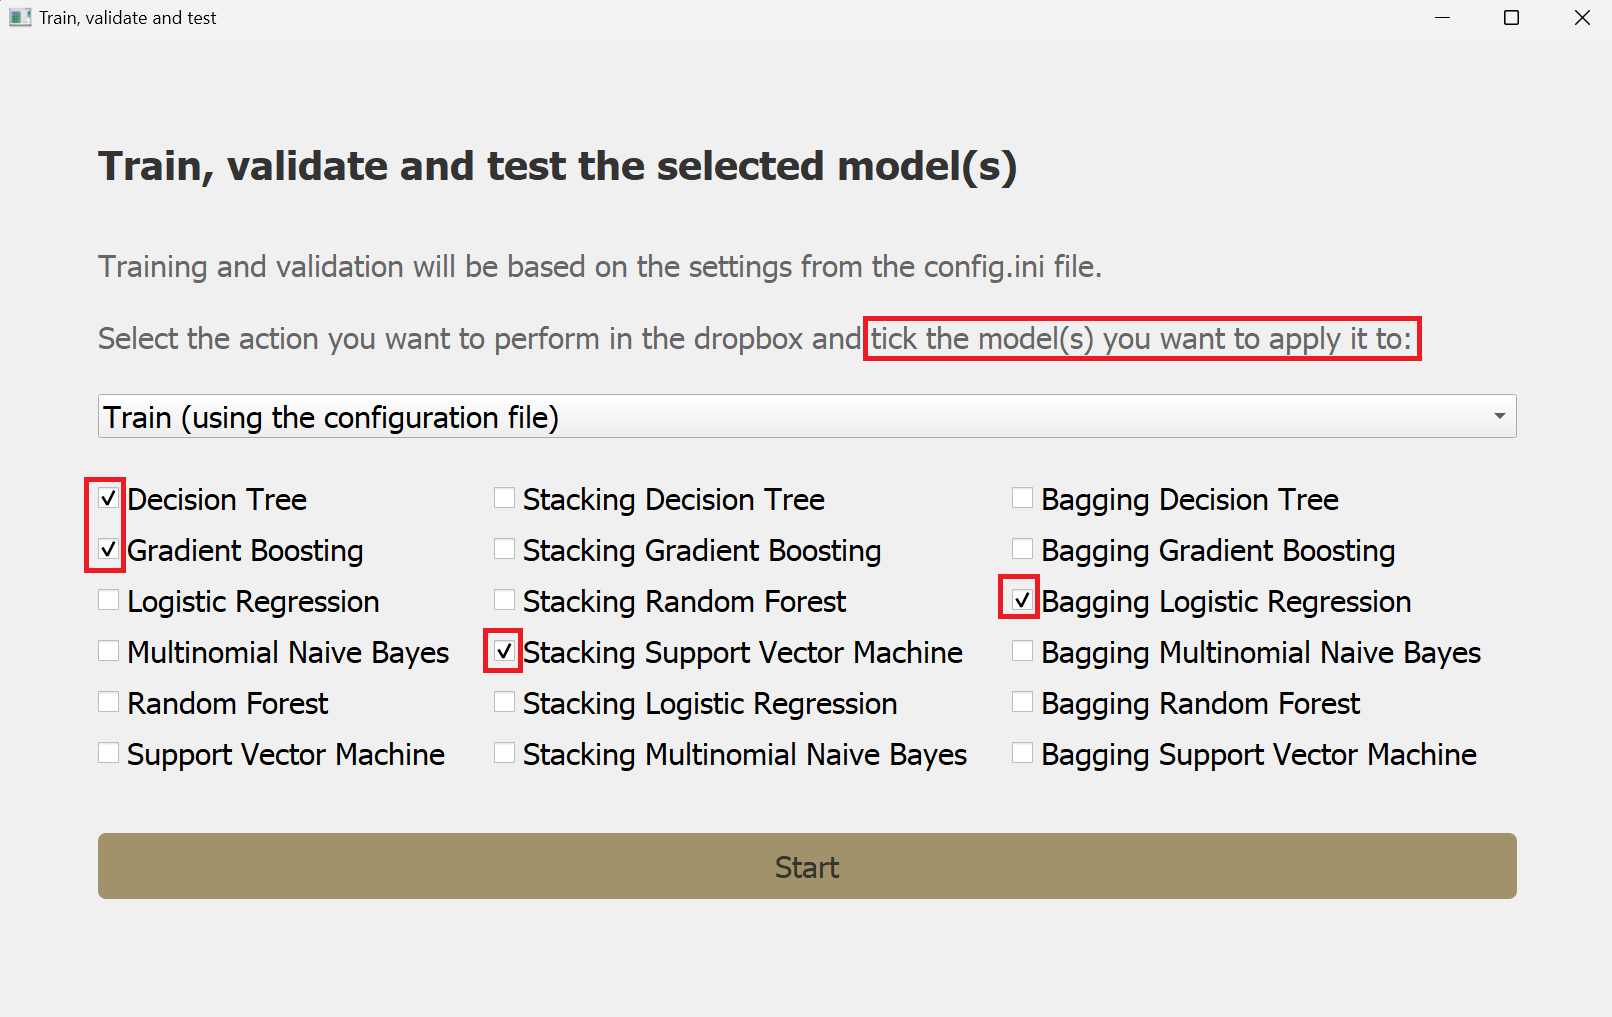
\includegraphics[width=16cm]{Images/Usage/Local/Train-Test-Validate-Window1.png}
\end{center}
\begin{center}
    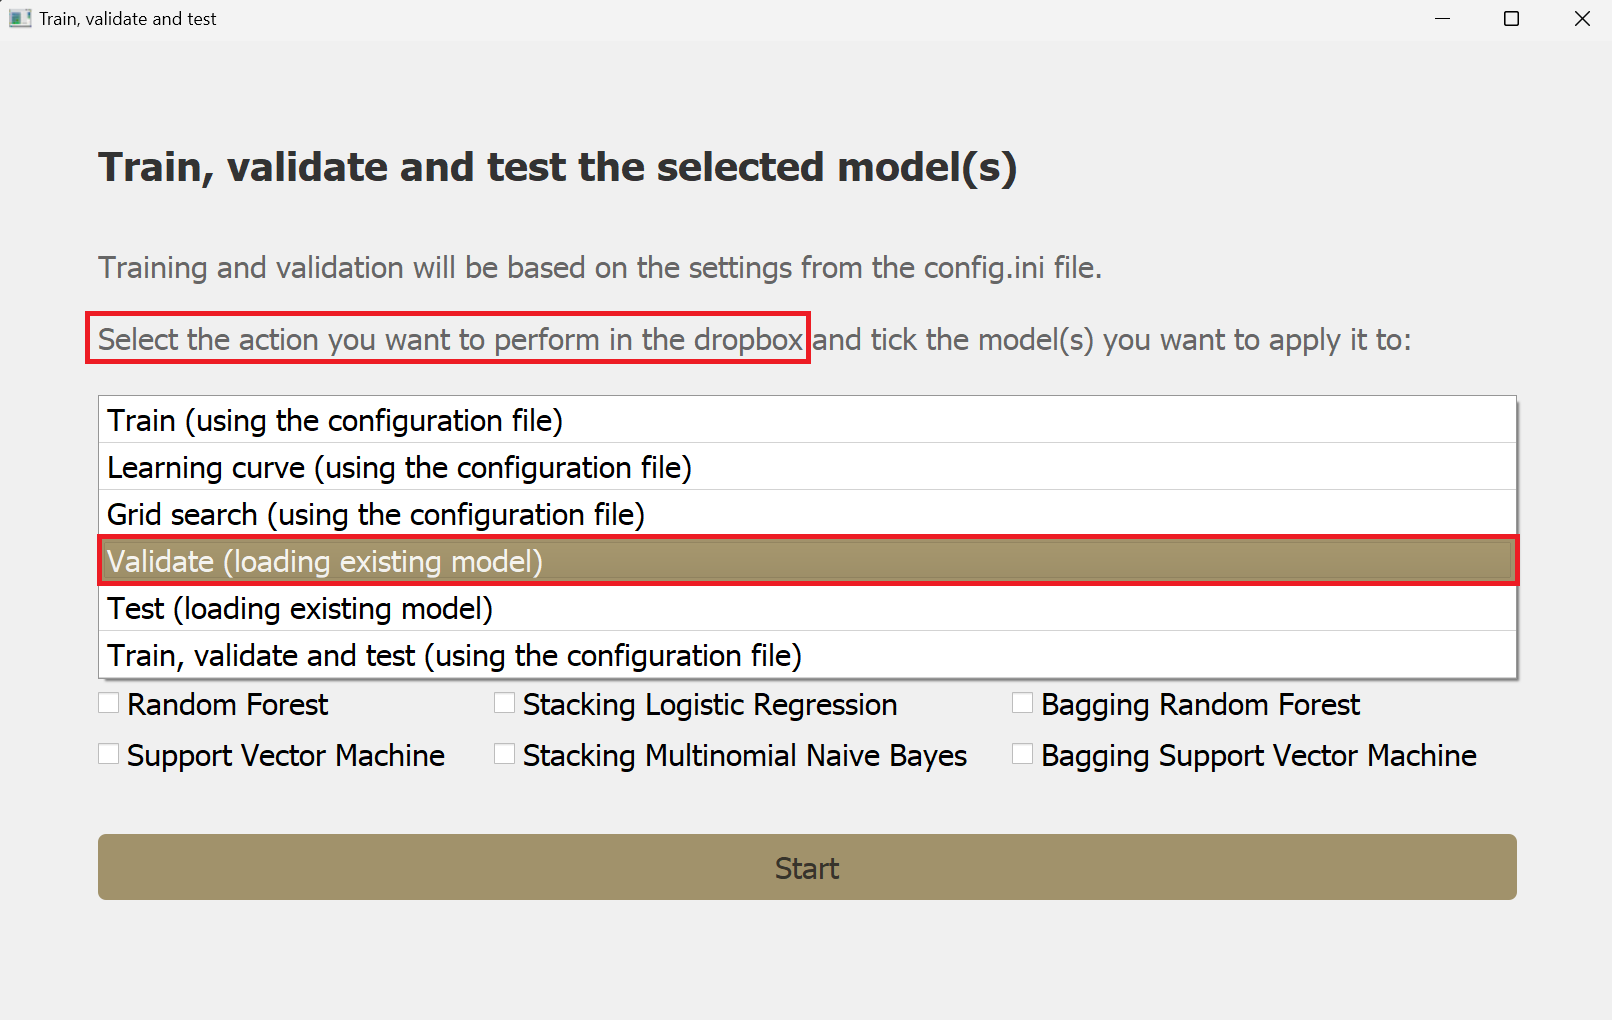
\includegraphics[width=16cm]{Images/Usage/Local/Train-Test-Validate-Window2.png}
\end{center}
\subsubsection{Detect Origin}
In the detect origin sub-window you will be able to select the model you want to use to perform the authorship detection task with. Copy and paste the text you want to analyze into the corresponding text box. Then press the \texttt{Detect Origin} button and wait for the task to finish. A new window will open with the result.
\begin{center}
    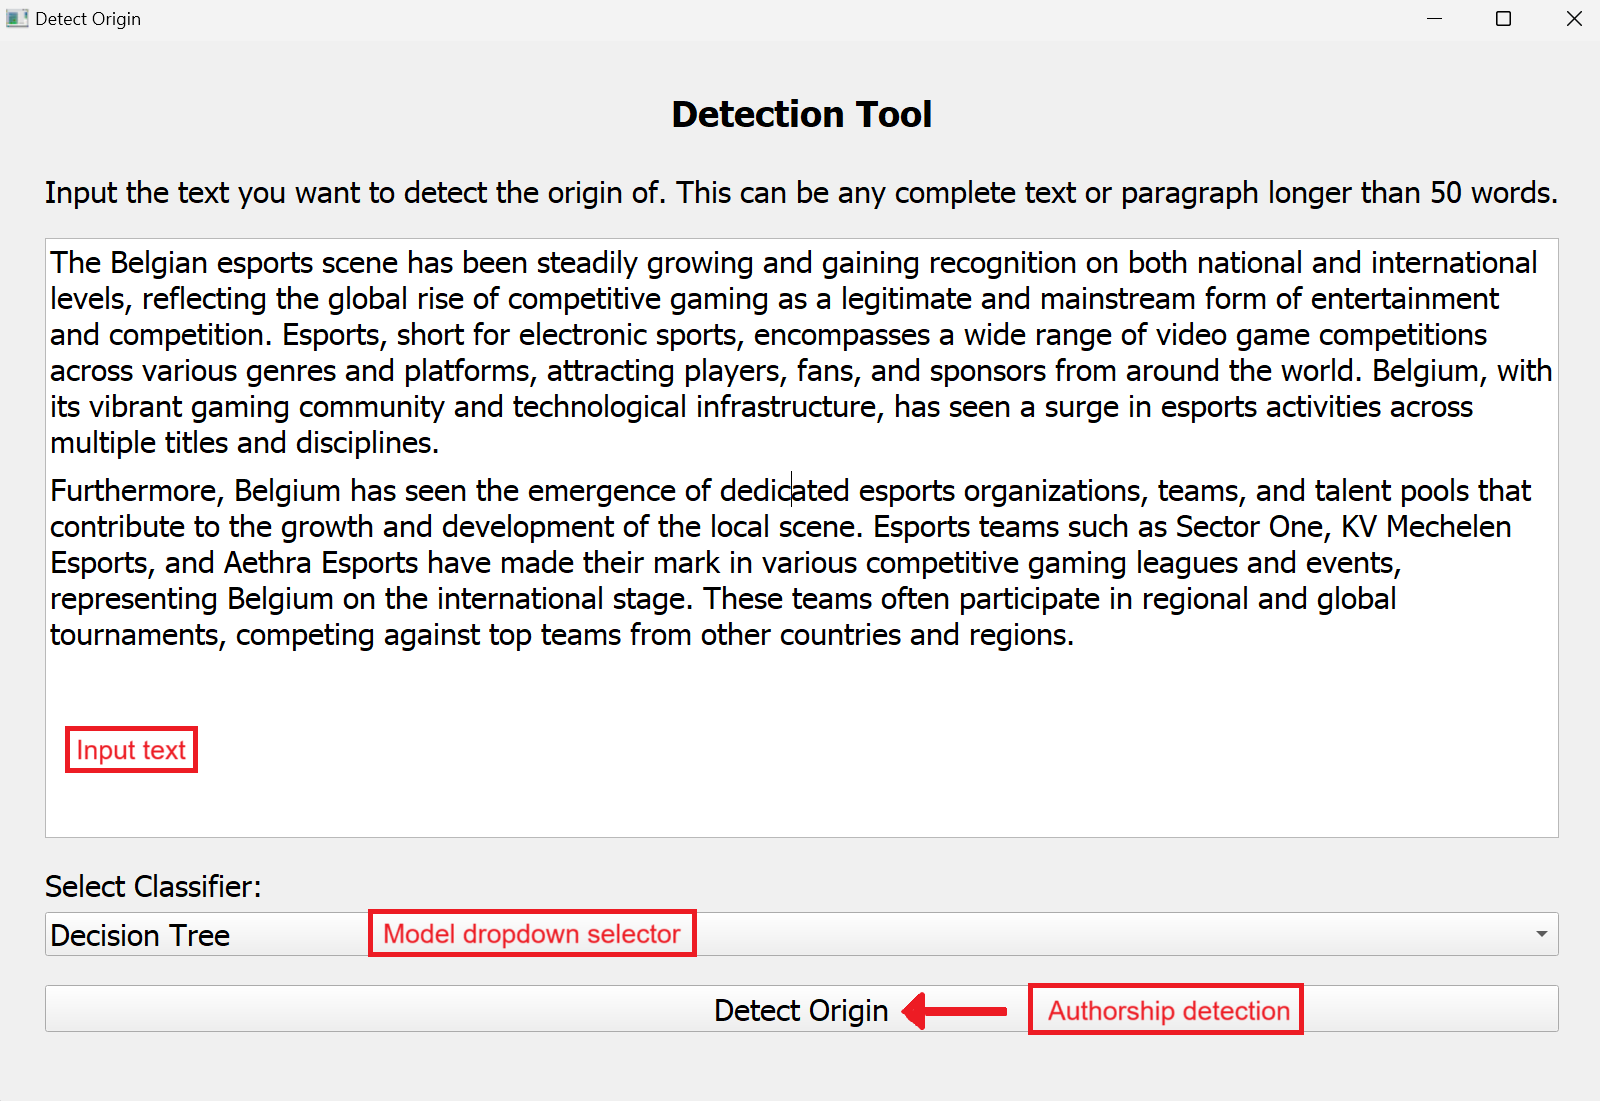
\includegraphics[width=17cm]{Images/Usage/Local/Detect-Origin-Window.png}
\end{center}
\clearpage
\subsection{Web based application}
The web application has a simplified interface. It contains text guidance on how to use the authorship detection feature, a text box to input the text to be analyzed and a button to start the process.
\begin{center}
    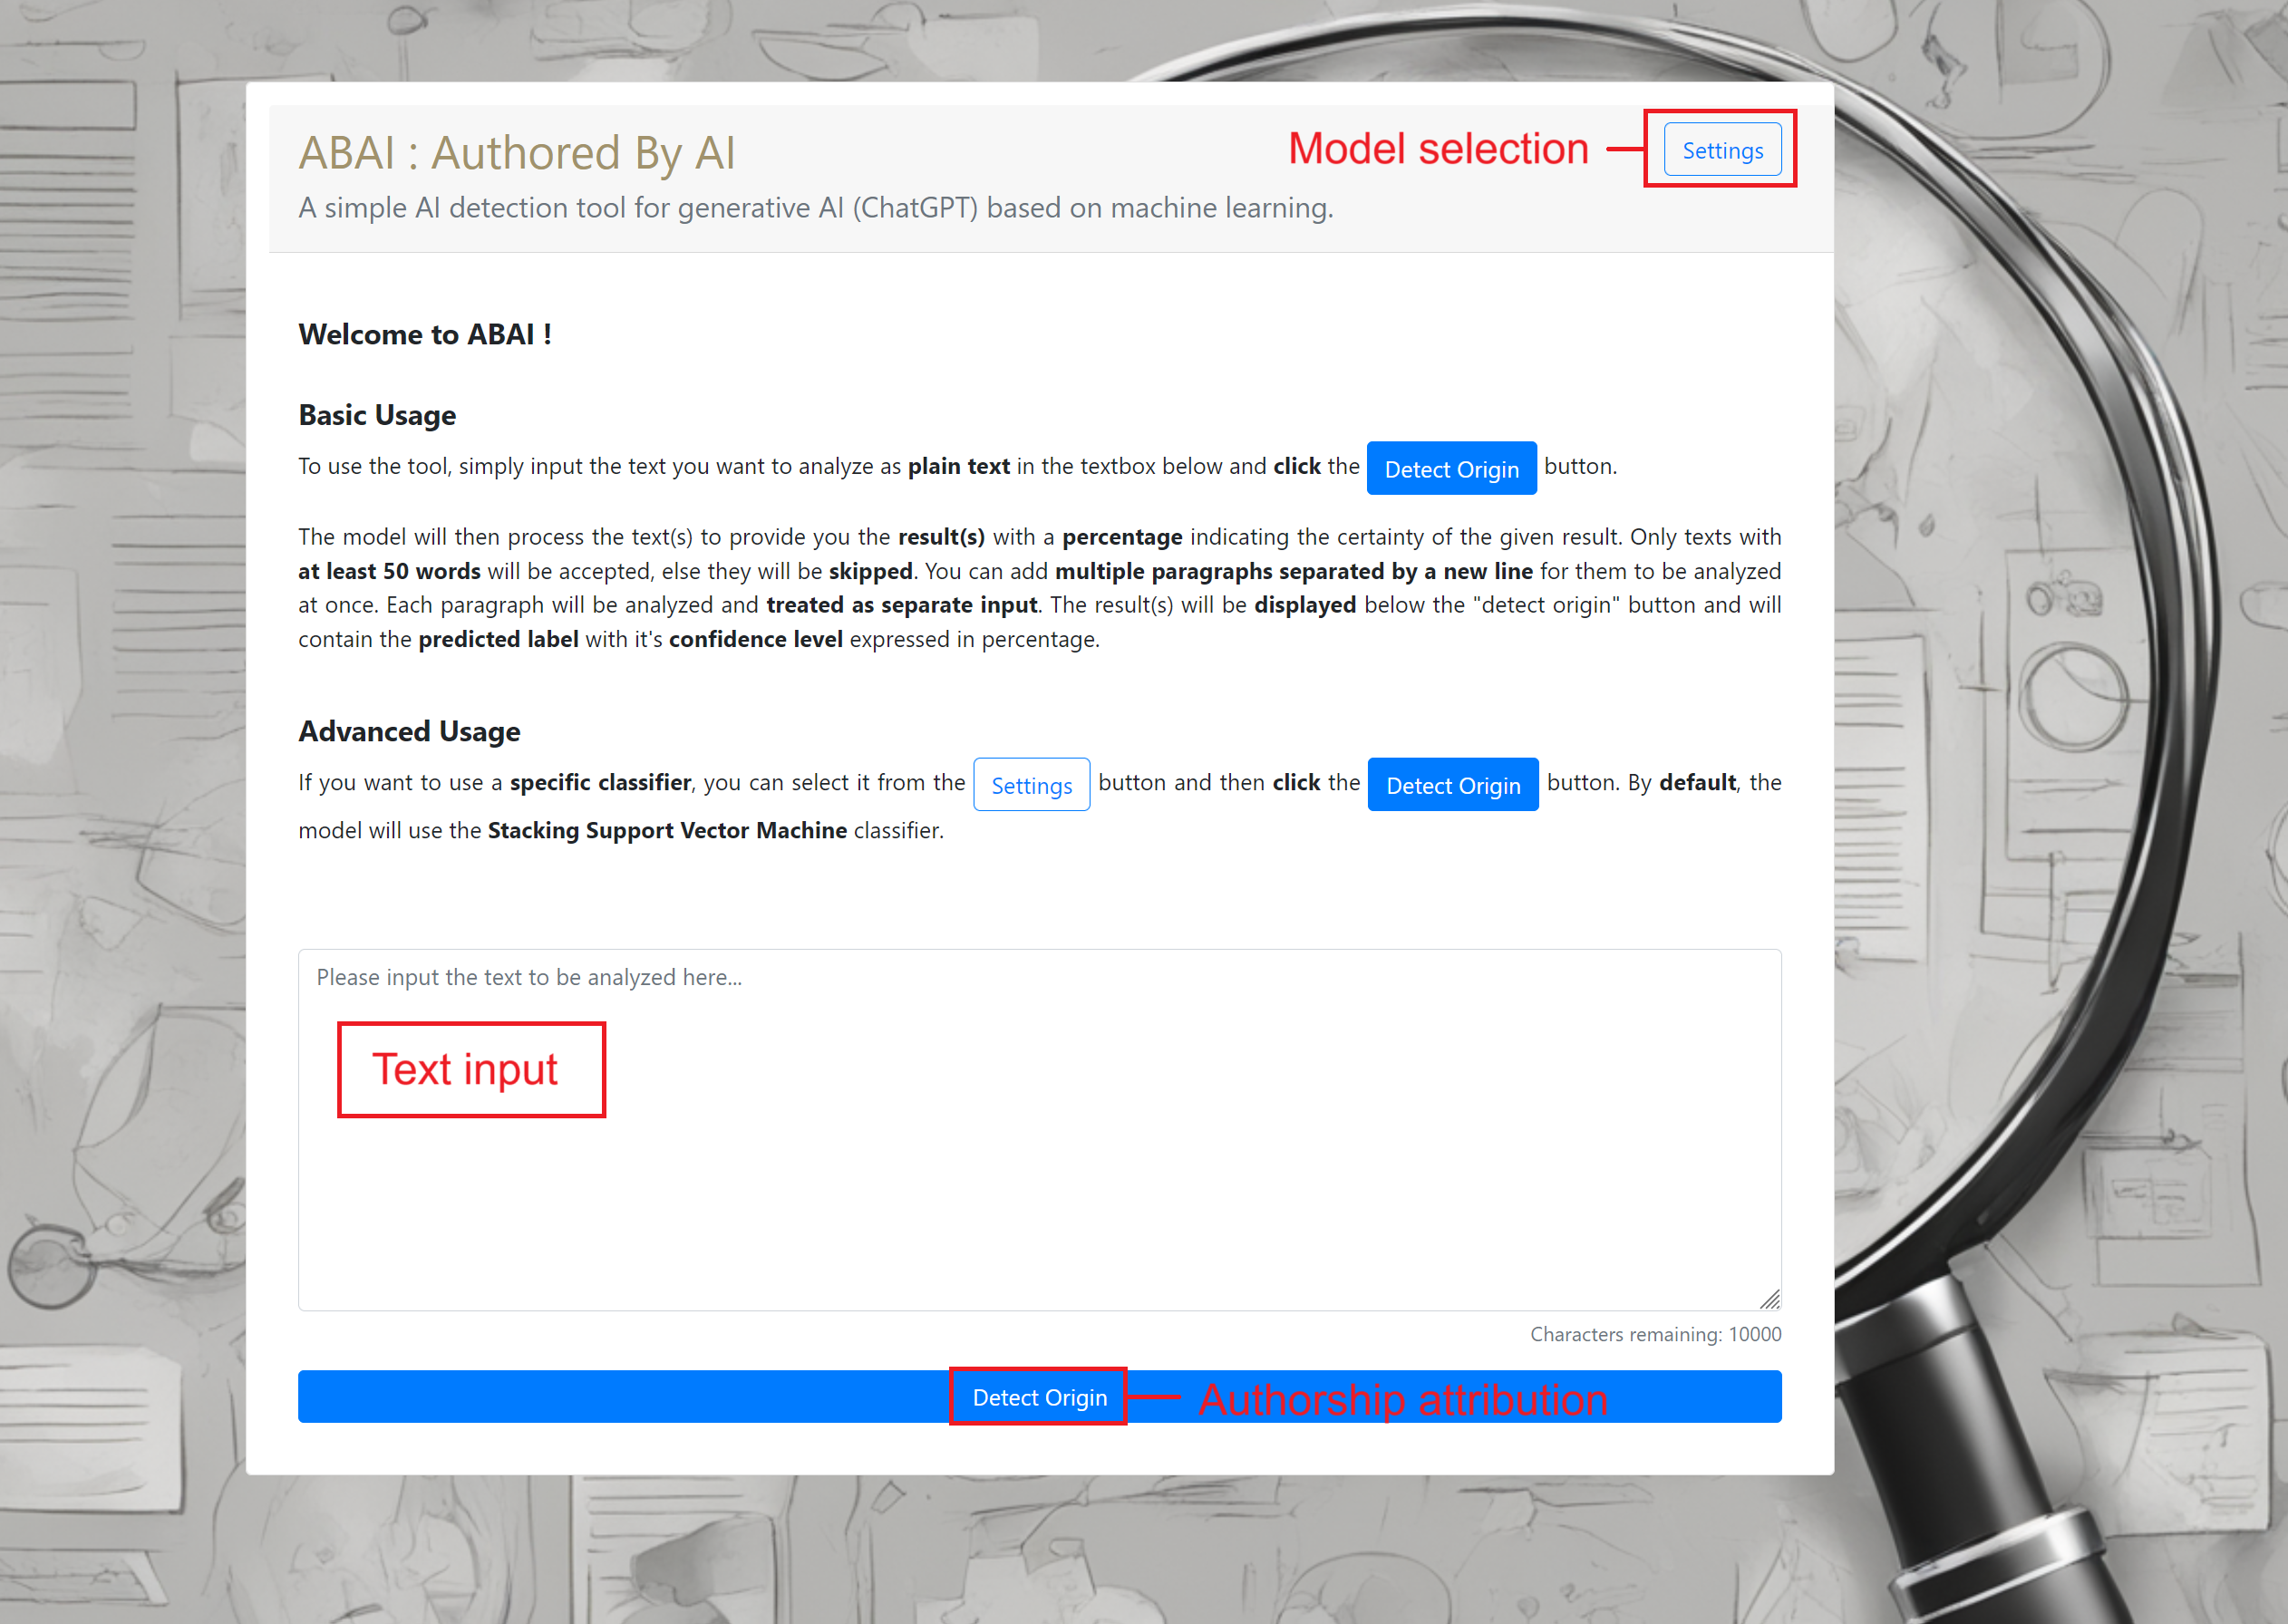
\includegraphics[width=17cm]{Images/Usage/Web/Web-application.png}
\end{center}
For a comparison between the different pre-trained models, the advanced usage let's you select a different model than the default one (Stacking Support Vector Machine). You do this by pressing the settings button situated in the top-right corner of the interface.
\begin{center}
    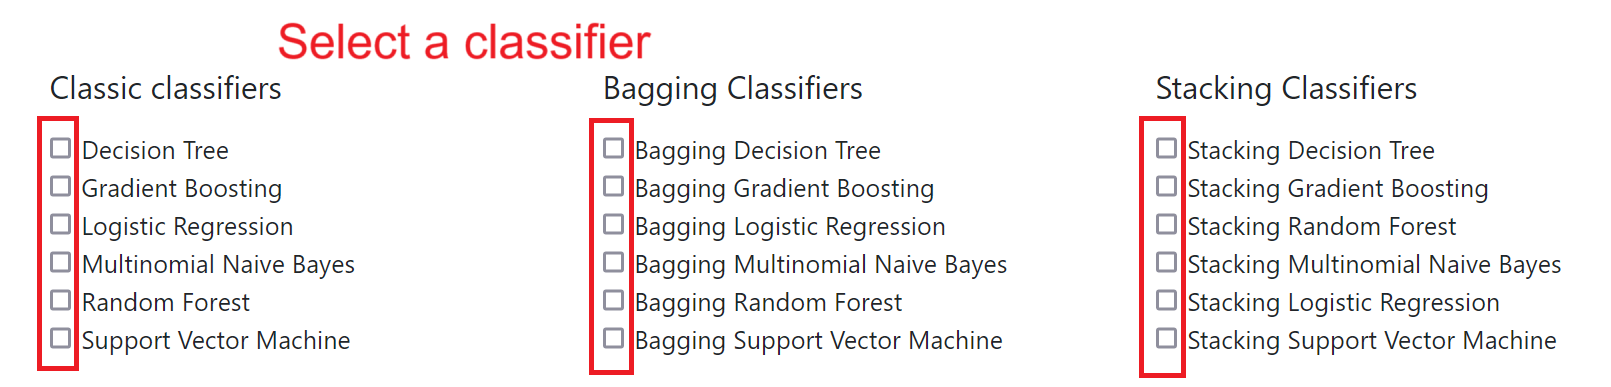
\includegraphics[width=17cm]{Images/Usage/Web/Web-settings.png}
\end{center}
When ready, press the \texttt{detect origin} button and wait for the results to be displayed bellow the \texttt{Detect Origin button}.
\begin{center}
    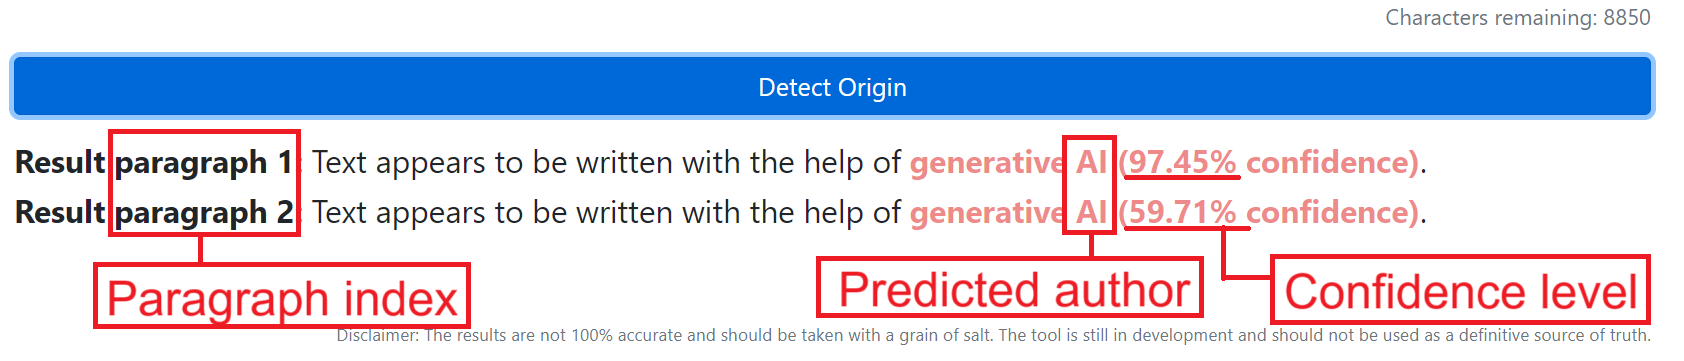
\includegraphics[width=17cm]{Images/Usage/Web/Web-results.png}
\end{center}

\subsection{How to guides}
\subsubsection{How to use the web/local application to detect the author of a given text?}
\begin{enumerate}
    \item Open the \hyperref[subsubsec:Web application]{web-based} version of the application or launch the \hyperref[subsubsec:Local application]{local} application using the appropriate method from the \hyperref[subsec:First steps]{installation} steps.
    
    \item Once the application started, locate the \textbf{input box} (navigate to the \texttt{Detect Origin} window for the local application) where you can paste the text to be analyzed. Copy the text you want to analyze and paste it there. Ensure that the text does not exceed the maximum \textbf{10 000 character limit} for the web application. 
    \begin{center}
        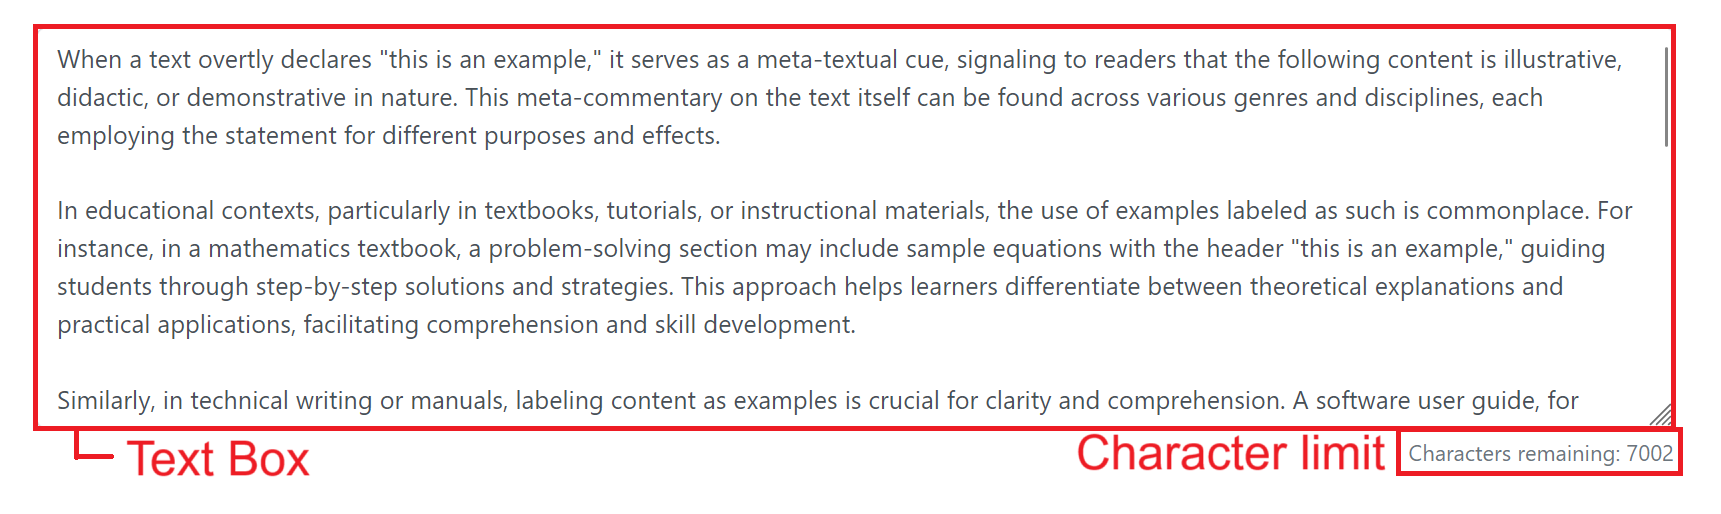
\includegraphics[width=17cm]{Images/Usage/Demo/Paste-limit.png}
    \end{center}
    \item After pasting the text, look for the \texttt{Detect Origin} button and click it to initiate the analysis process.
    \begin{center}
        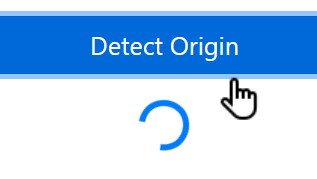
\includegraphics[width=4cm]{Images/Usage/Demo/Detect-load.png}
    \end{center}
    \item Wait for the analysis to complete. Depending on the complexity of the text and the processing steps, this may take a few moments.
    \item Once the analysis is finished, review the results displayed by the application. The results will indicate whether the text is likely to be authored by a human or generated by an AI model with a certain level of confidence. The result will also indicate if a paragraph doesn't meet a requirement like word length.
\begin{center}
    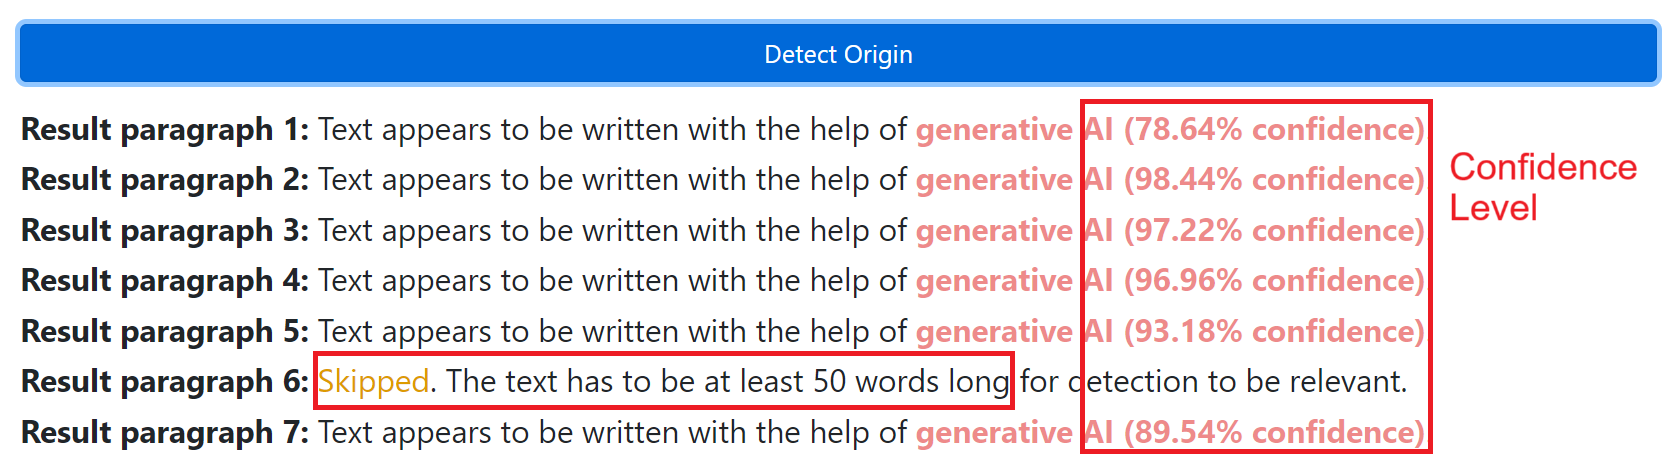
\includegraphics[width=16cm]{Images/Usage/Demo/Results.png}
\end{center}
\end{enumerate}

\subsubsection{How to use the local application to add local texts to the dataset?}
\begin{enumerate}
    \item Open the \hyperref[subsubsec:Web application]{web-based} version of the application or launch the \hyperref[subsubsec:Local application]{local} application using the appropriate method from the \hyperref[subsec:First steps]{installation} steps.
    \item Navigate from the main menu to the \hyperref[subsubsec:database]{Database} sub-window.
    \begin{center}
        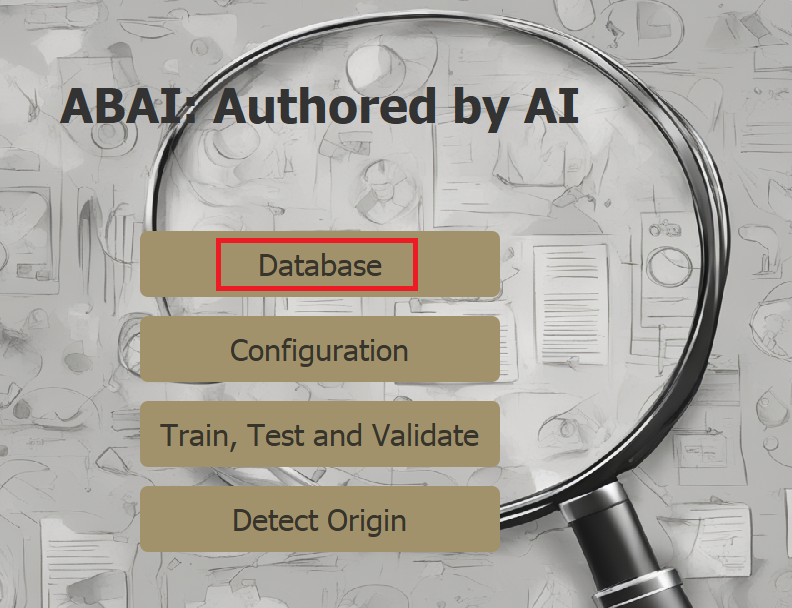
\includegraphics[width=16cm]{Images/Usage/Demo/navigate-database.png}
    \end{center}
    \item On the database sub-window select the button to add a text to the local texts with the corresponding label (human or AI).
    \begin{center}
        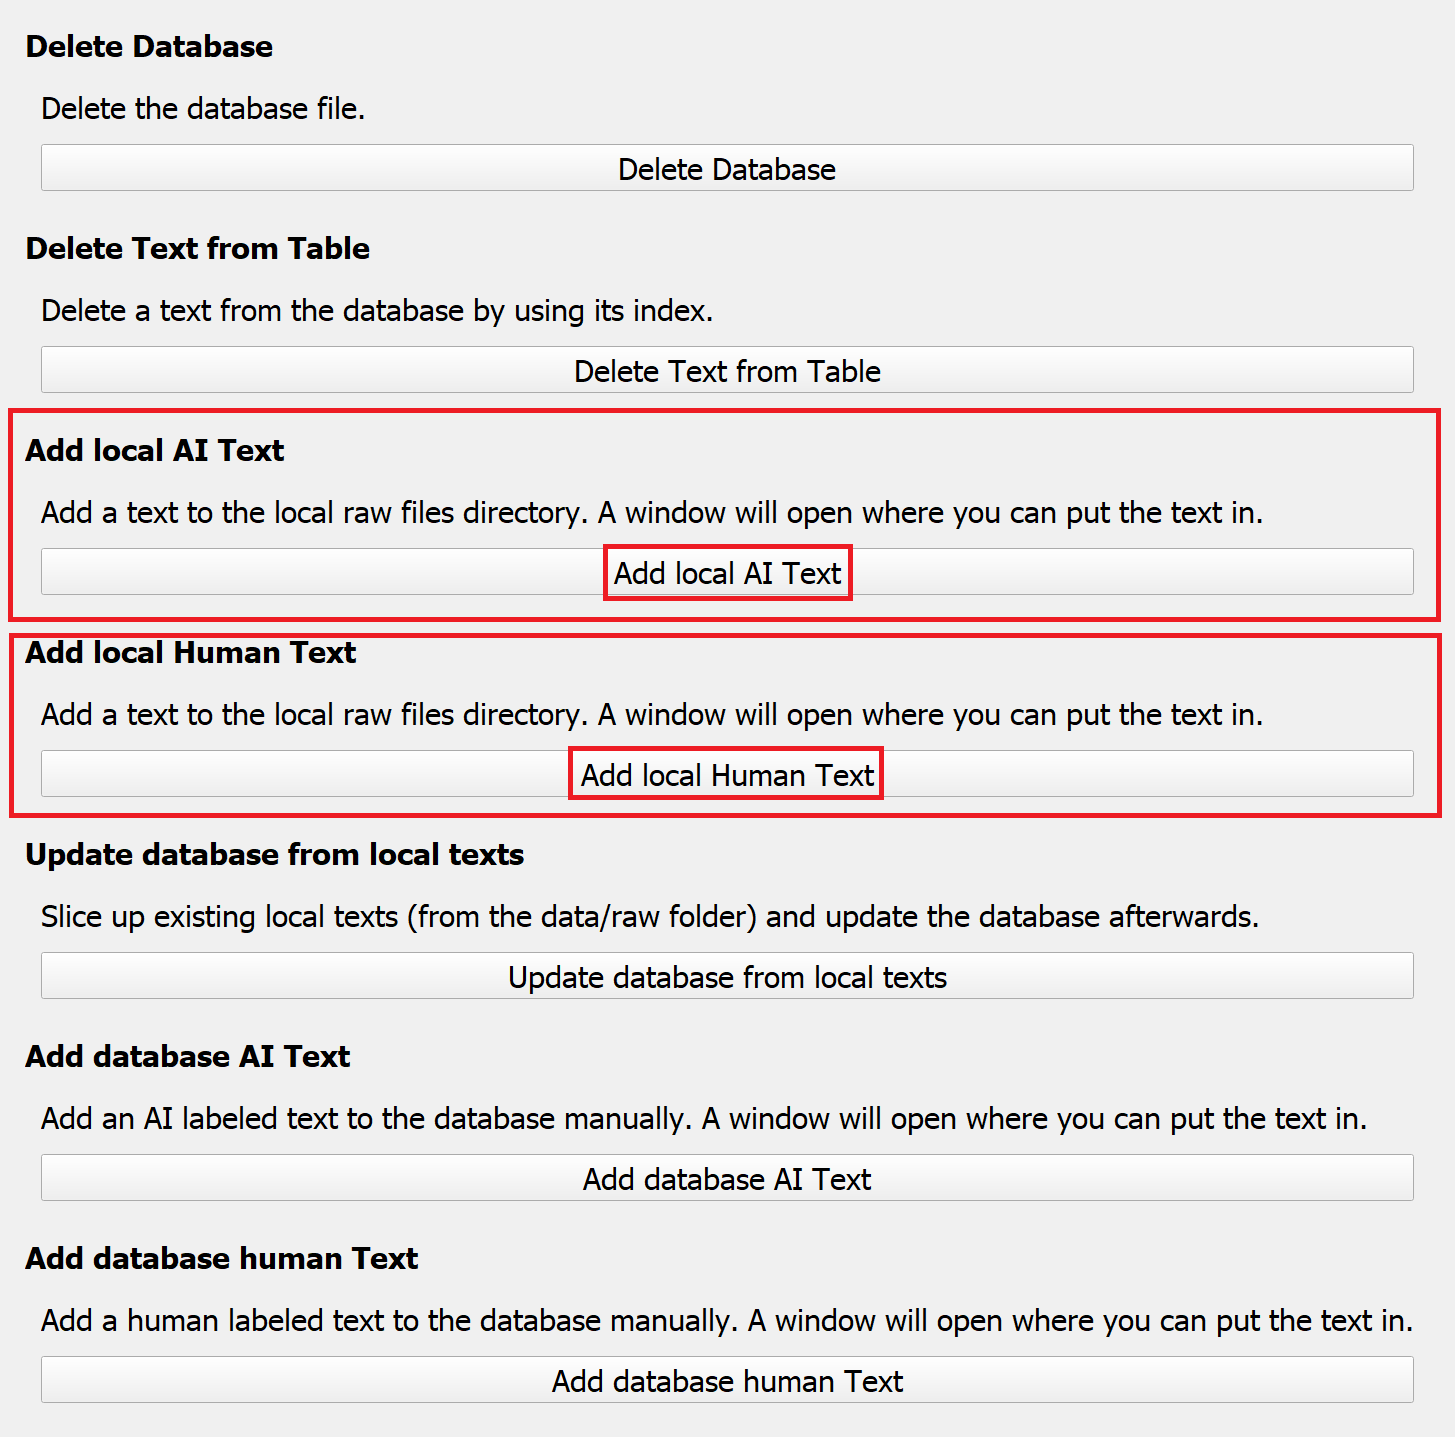
\includegraphics[width=14cm]{Images/Usage/Demo/Add-local.png}
    \end{center}
    \item Paste the text into the text box and click the \textbf{\texttt{OK}} button to save.
    \begin{center}
        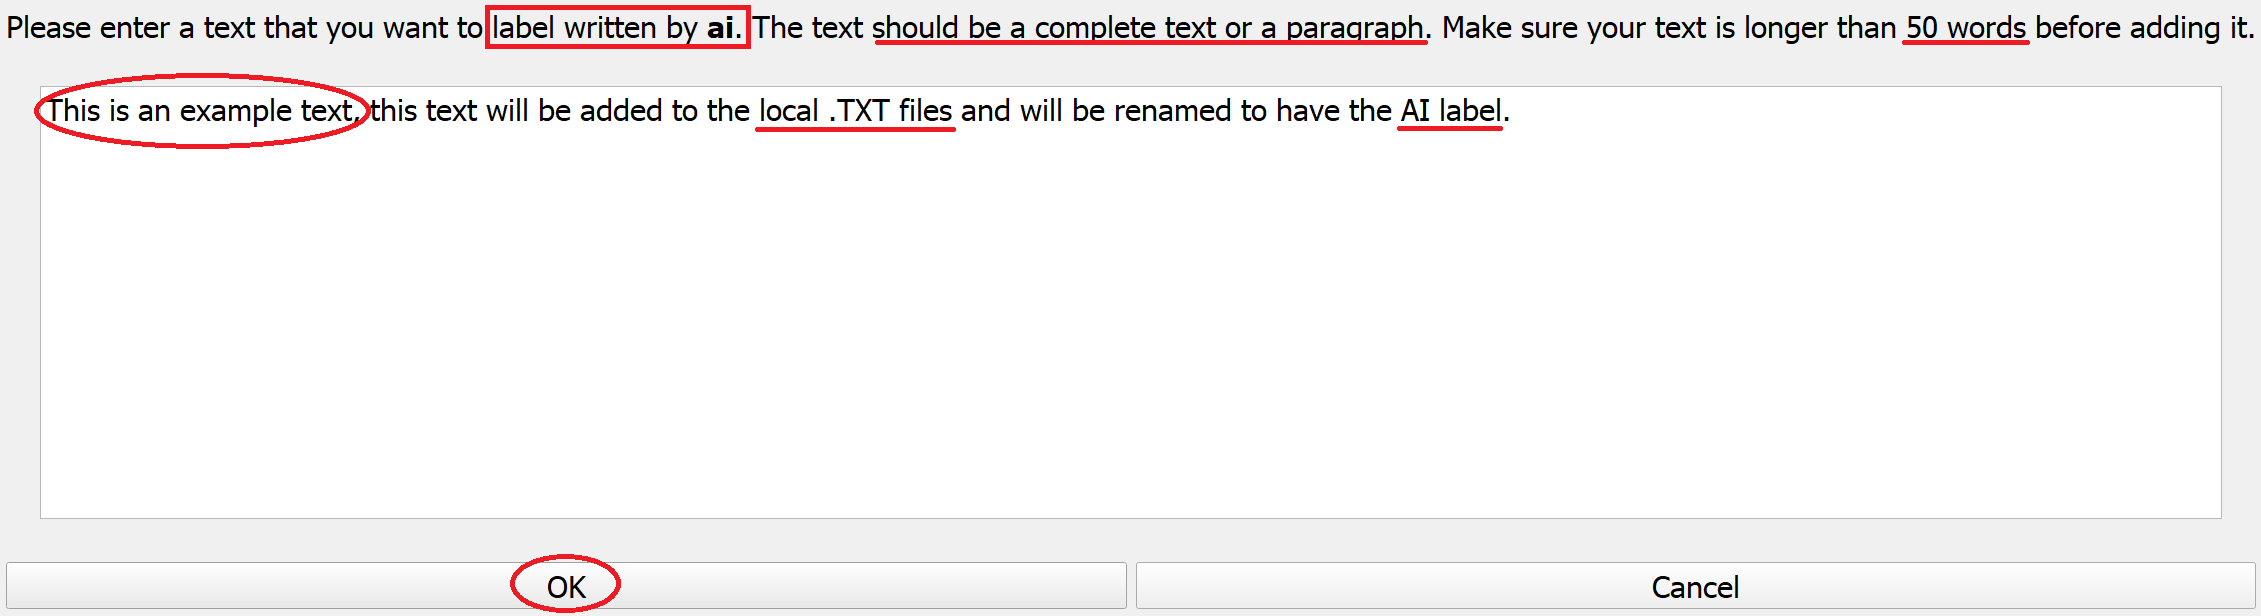
\includegraphics[width=16.5cm]{Images/Usage/Demo/Add-AI.png}
    \end{center}
    \clearpage
    \item Navigate back to the \hyperref[subsubsec:database]{Database} sub-window and click on the \texttt{Update database from local texts} button to include the freshly added local texts in the database.
    \begin{center}
        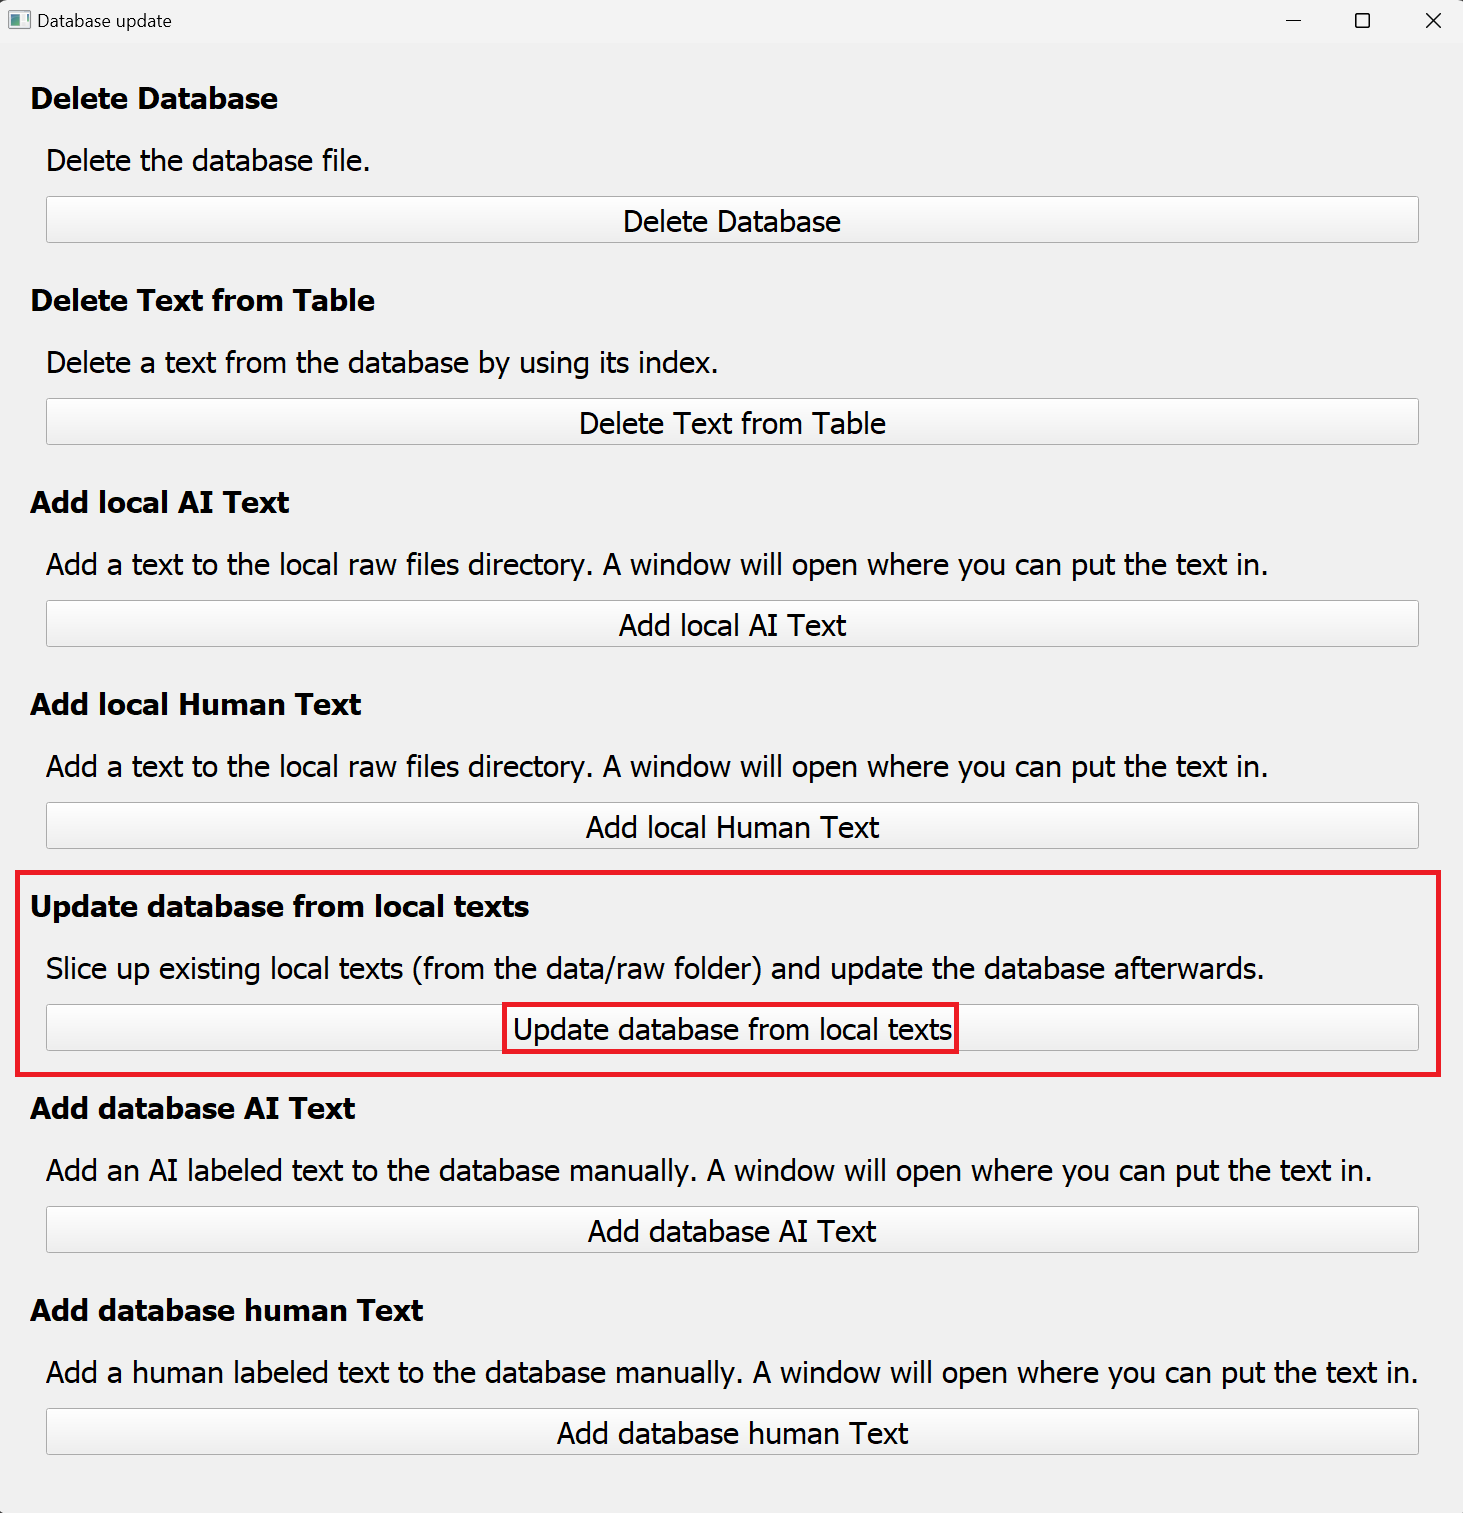
\includegraphics[width=16.5cm]{Images/Usage/Demo/Update-database.png}
    \end{center}
\end{enumerate}
\clearpage
\subsubsection{How to use the local application to delete texts from the dataset?}
\begin{enumerate}
    \item Open the \hyperref[subsubsec:Web application]{web-based} version of the application or launch the \hyperref[subsubsec:Local application]{local} application using the appropriate method from the \hyperref[subsec:First steps]{installation} steps.
    \item Navigate from the main menu to the \hyperref[subsubsec:database]{Database} sub-window.
    \begin{center}
        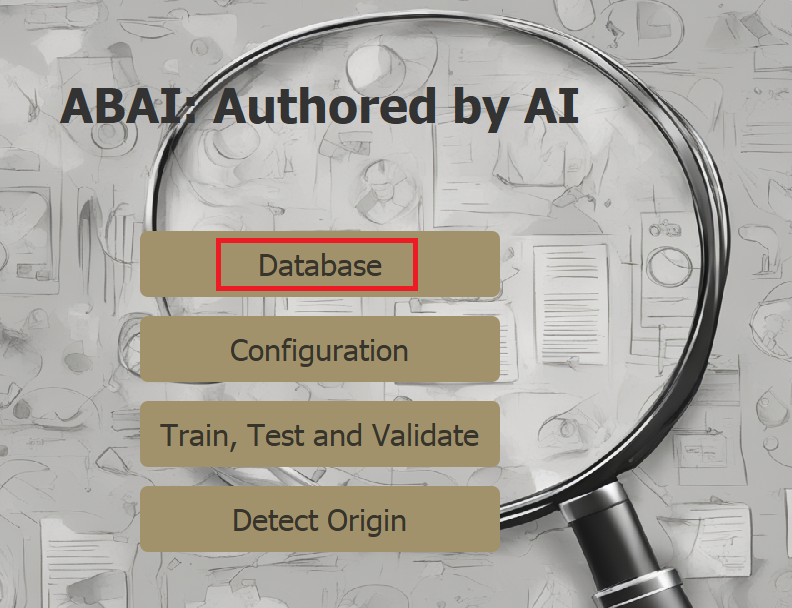
\includegraphics[width=11cm]{Images/Usage/Demo/navigate-database.png}
    \end{center}
    \item On the database sub-window select the button \texttt{Delete Text from Table}.
    \begin{center}
        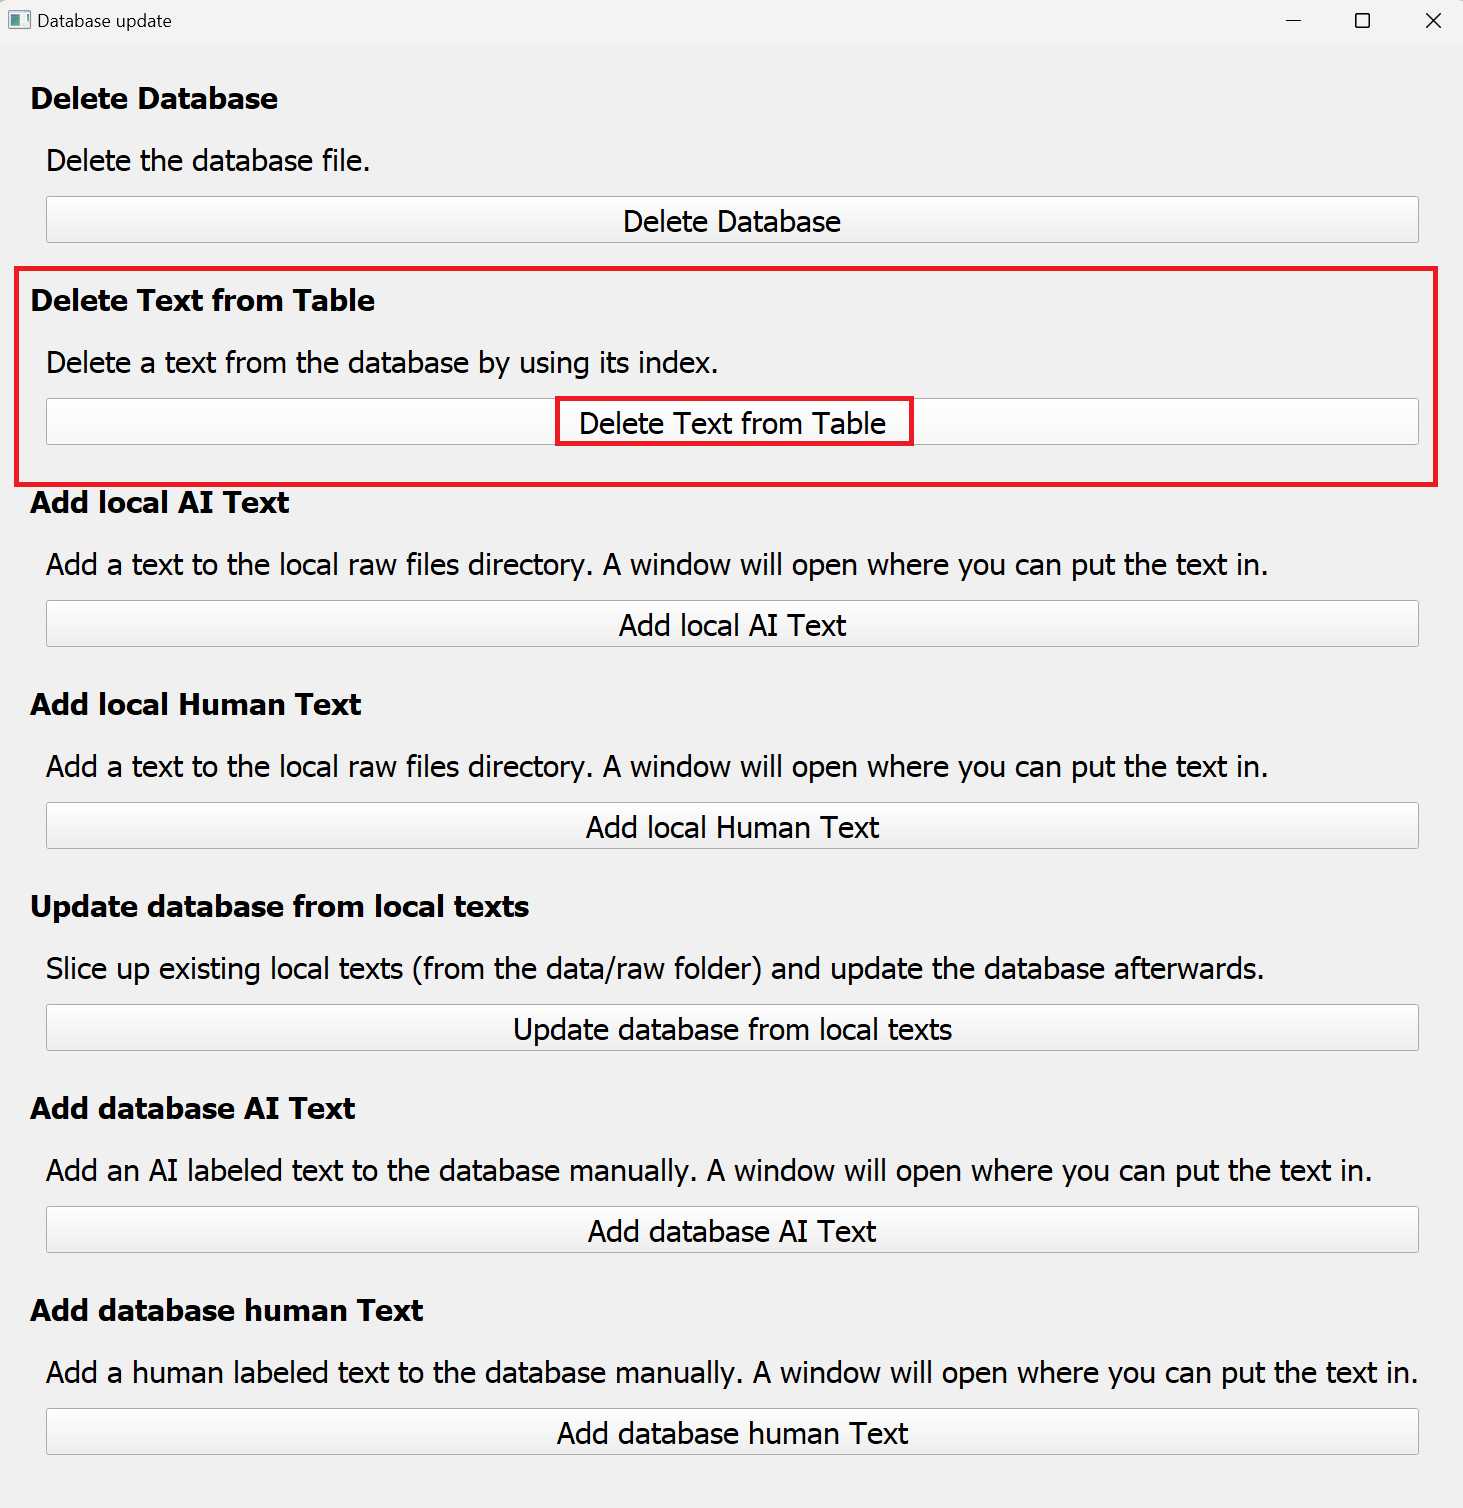
\includegraphics[width=11cm]{Images/Usage/Demo/delete.png}
    \end{center}
    \item On the newly opened deletion window, select the text to delete from the preview list by ticking the corresponding box and then click on the \texttt{Delete Selected} button to confirm. Deletion will output the result under the preview panel.
    \begin{center}
        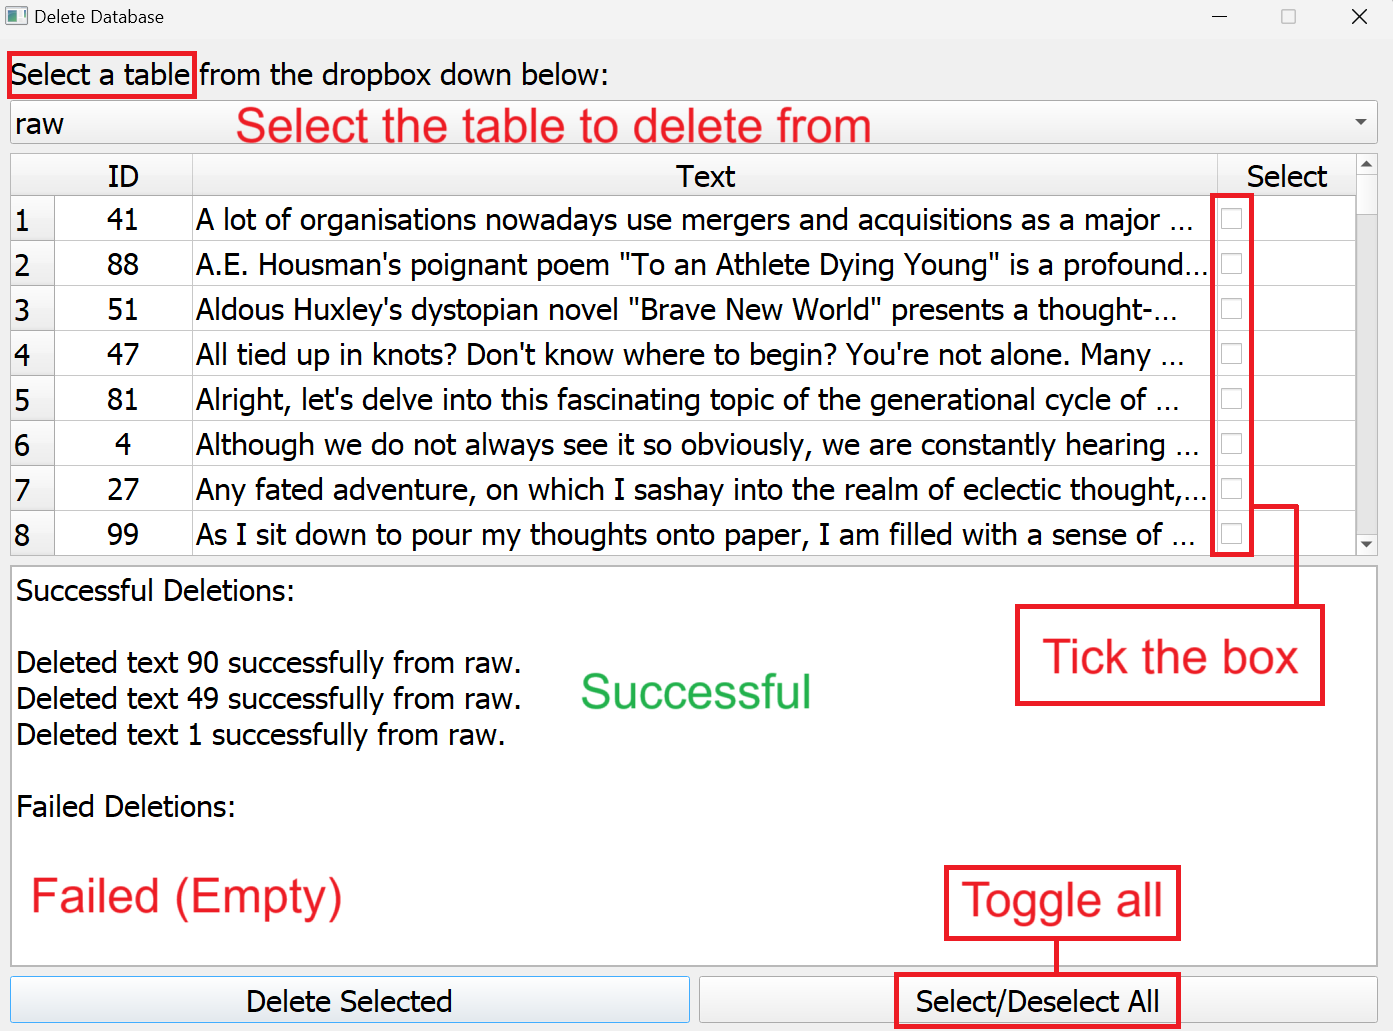
\includegraphics[width=16.5cm]{Images/Usage/Demo/Deletion.png}
    \end{center}
\end{enumerate}
\clearpage
\subsubsection{How to use the local application to train, test and validate models with a new configuration?}
\begin{enumerate}
    \item Open the \hyperref[subsubsec:Web application]{web-based} version of the application or launch the \hyperref[subsubsec:Local application]{local} application using the appropriate method from the \hyperref[subsec:First steps]{installation} steps.
    \item If you have the desired configuration, you can skip to step 4, else navigate to the \hyperref[subsubsec:configuration]{Configuration} sub-window.
    \begin{center}
        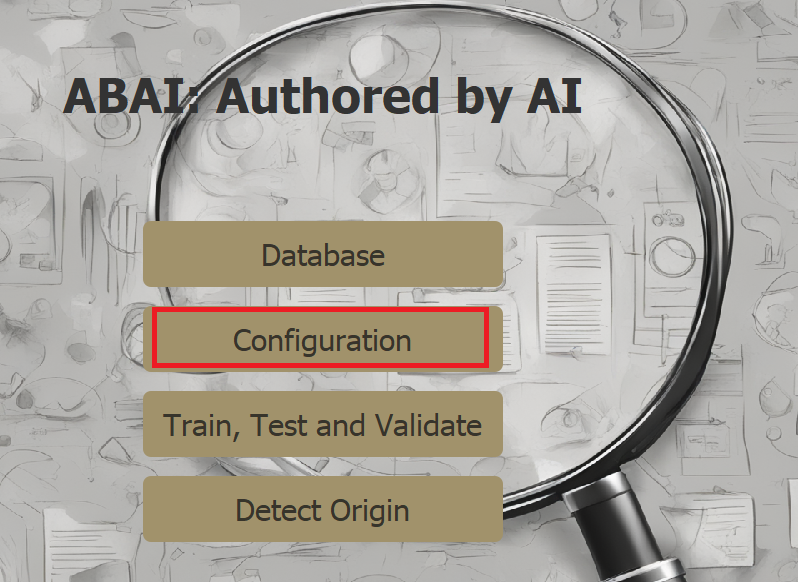
\includegraphics[width=10.5cm]{Images/Usage/Demo/config.png}
    \end{center}
    \item On the Configuration sub-window select the options (brief explanation \hyperref[subsubsec:config-brief-explain]{here}) you want. To illustrate this example, let's say we only want to keep all features extracted before pre-processing.
    \begin{center}
        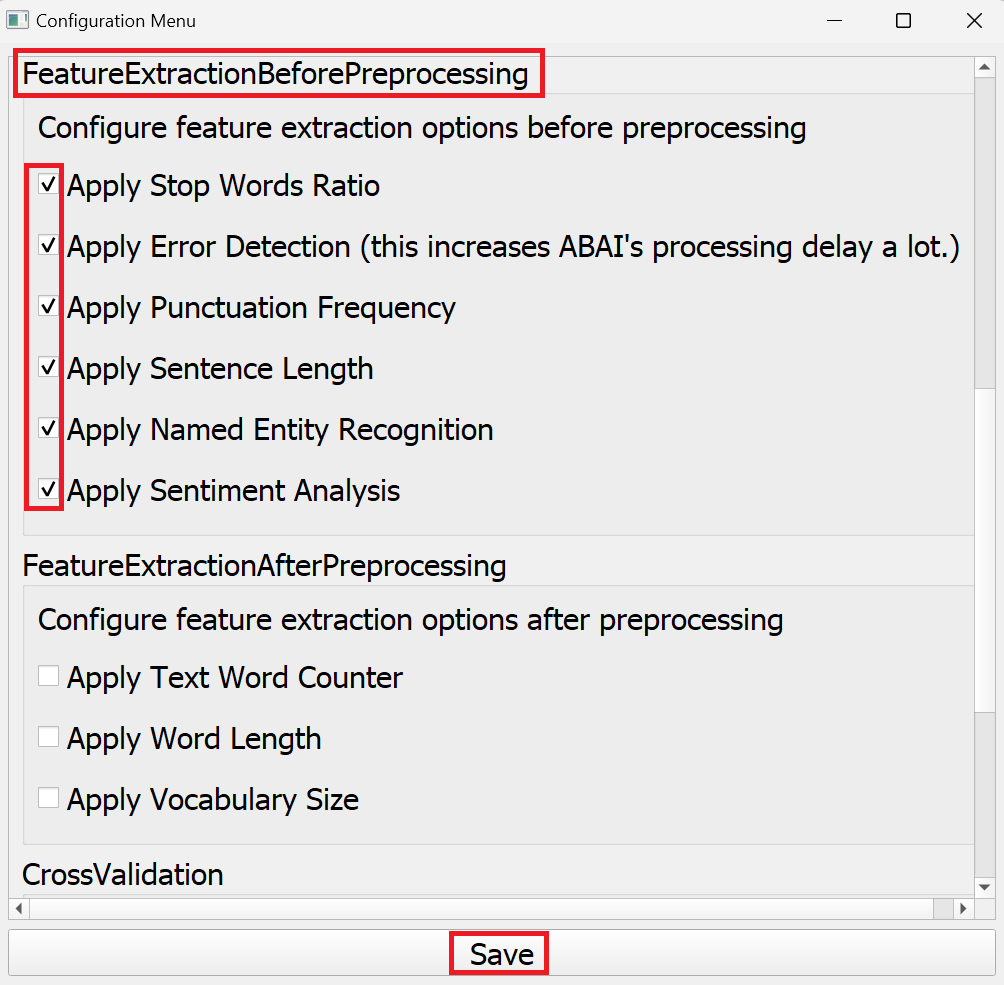
\includegraphics[width=10.5cm]{Images/Usage/Demo/train-config.png}
    \end{center}
    \item Navigate from the main menu to the \hyperref[subsubsec:train-test-validate]{Train, Test and Validate} sub-window.
    \begin{center}
        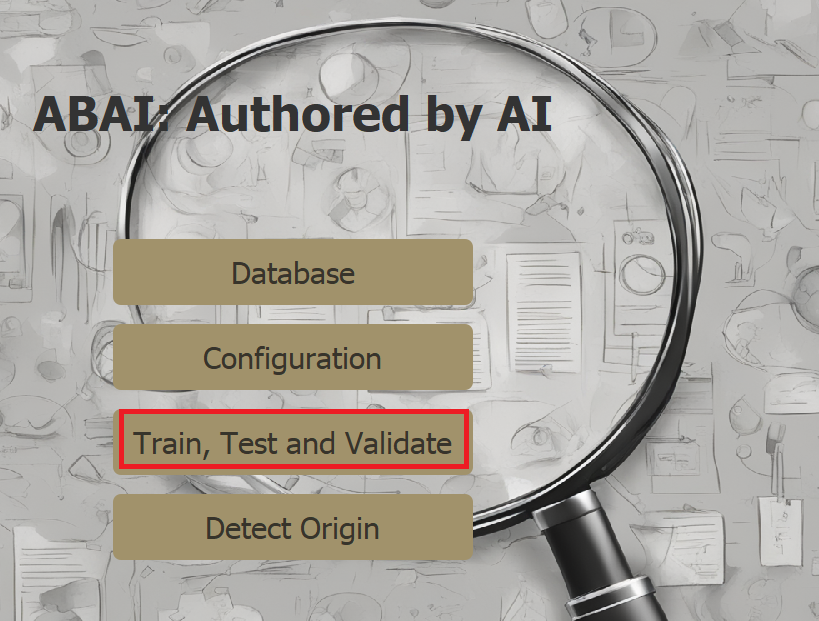
\includegraphics[width=14cm]{Images/Usage/Demo/train-test-validate.png}
    \end{center}
    \item On the Train, Test and Validate sub-window select the action you want to perform. For this how-to, select \texttt{Train, validate and test} from the dropdown list.
    \begin{center}
        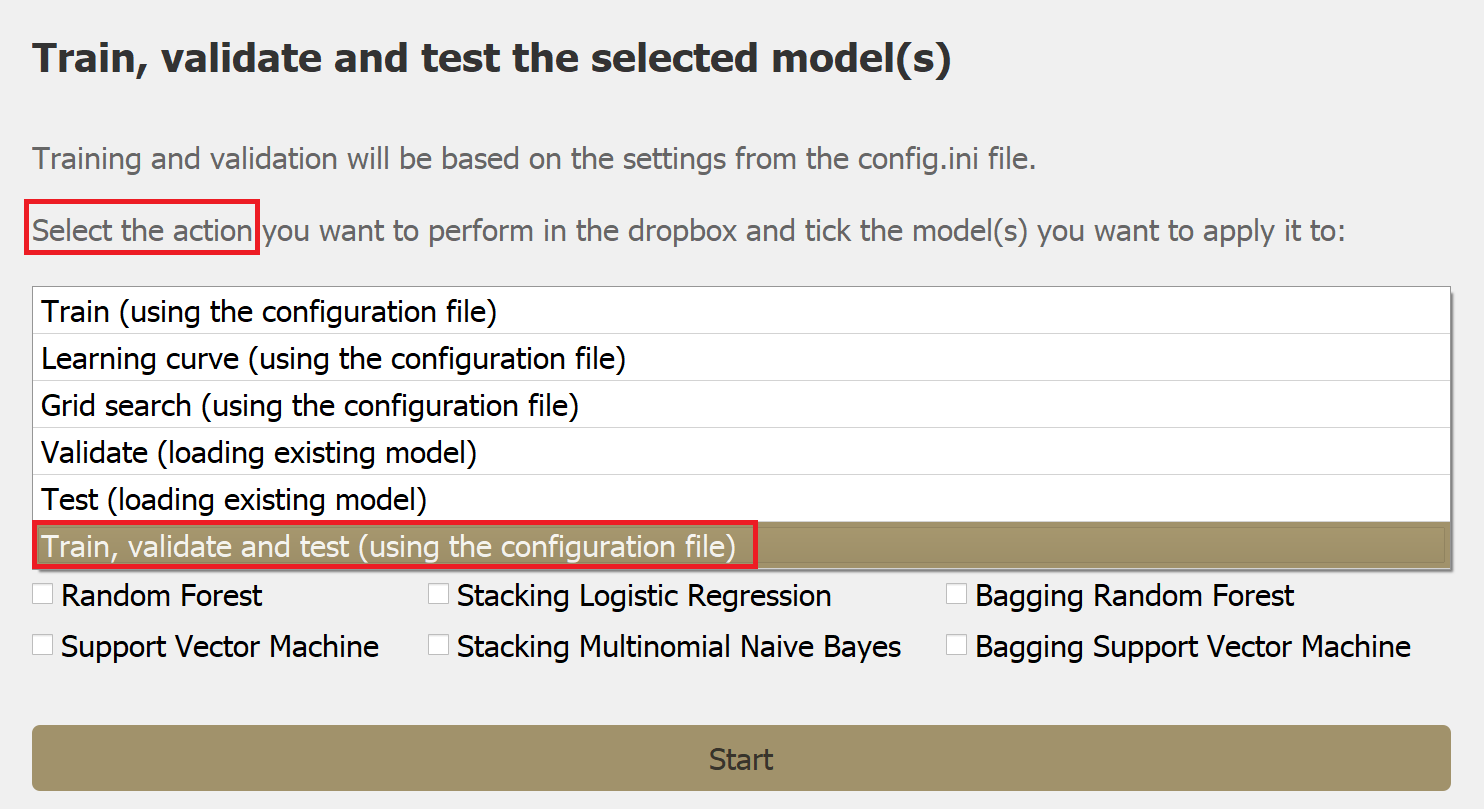
\includegraphics[width=14cm]{Images/Usage/Demo/train-select.png}
    \end{center}
    \clearpage
    \item On the same window, select the model(s) to perform the action on, by ticking the corresponding box and then click on the \texttt{Start} button to confirm. 
    \begin{center}
        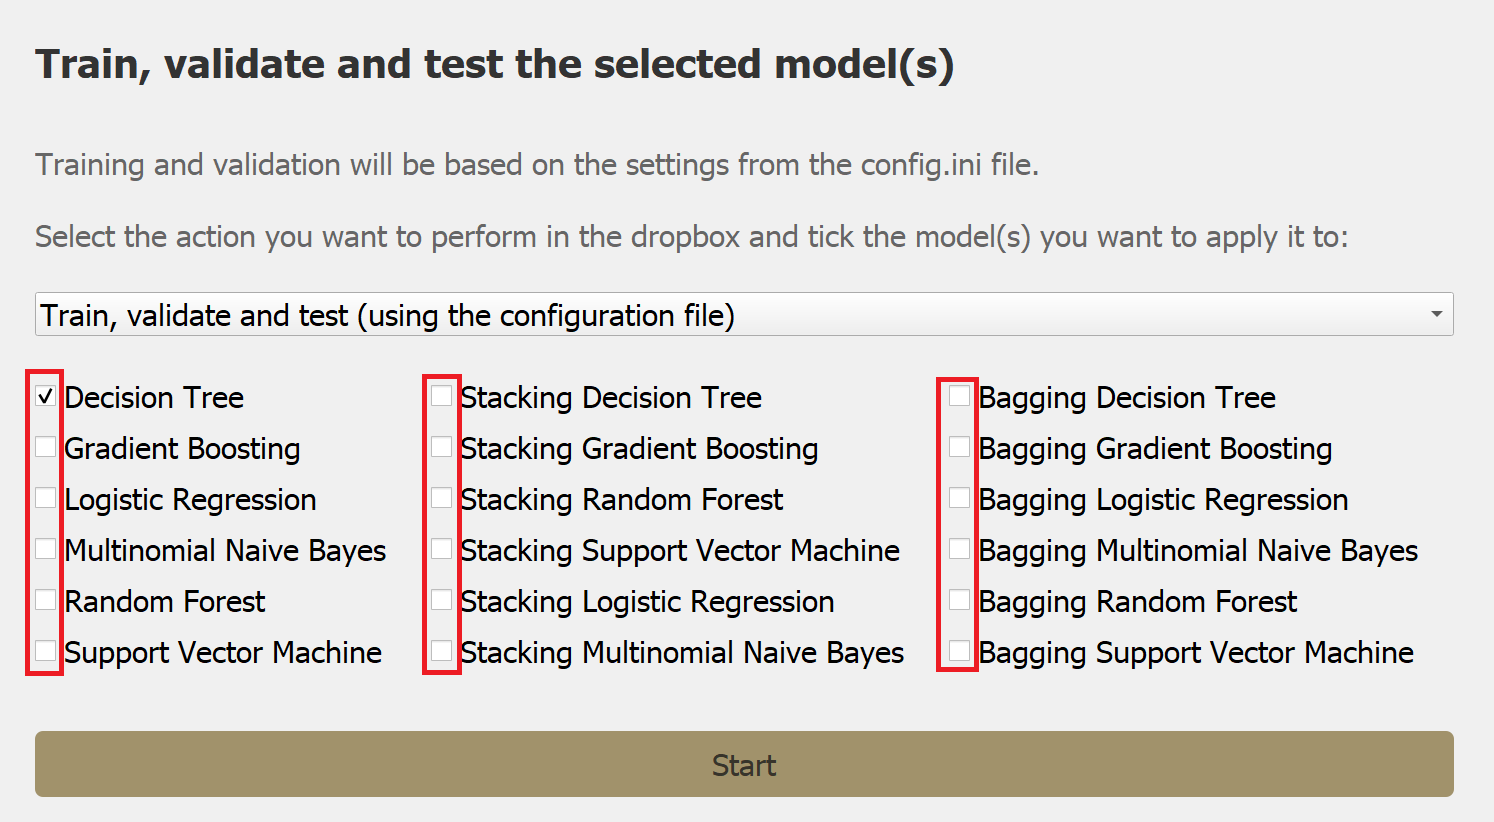
\includegraphics[width=14cm]{Images/Usage/Demo/train-model.png}
    \end{center}
    \item Please wait patiently for the action to finish, the window may look stuck for a while depending on the complexity of the action. When ready, a new window will open to display the results.
    \begin{center}
        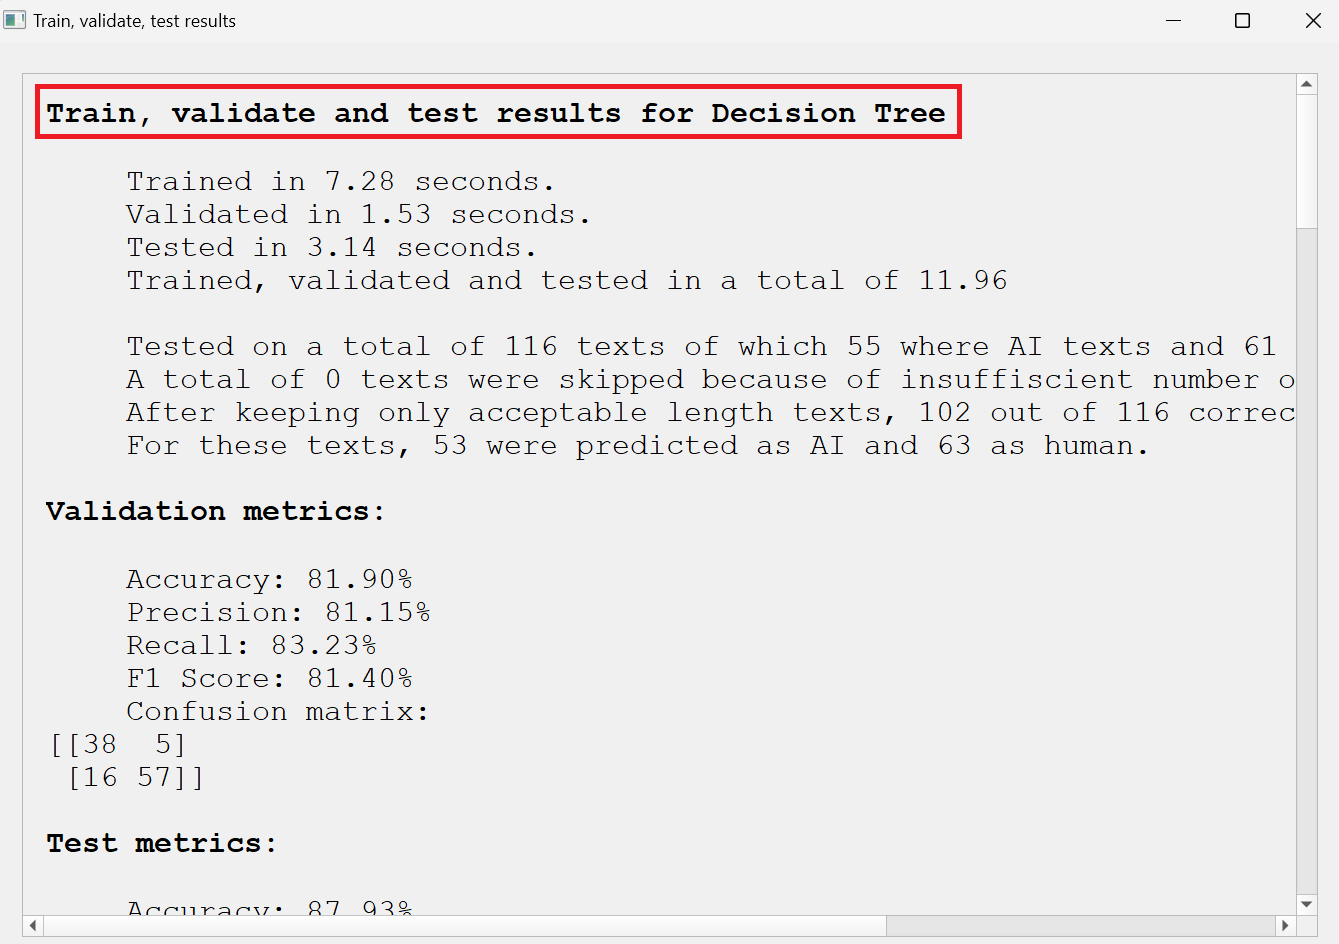
\includegraphics[width=14cm]{Images/Usage/Demo/train-result.png}
    \end{center}
\end{enumerate}